%%%%%%%%%%%%%%%%%%%%%%%%%%%%%%%%%%%%%%%%%
% Short Sectioned Assignment LaTeX Template Version 1.0 (5/5/12)
% This template has been downloaded from: http://www.LaTeXTemplates.com
% Original author:  Frits Wenneker (http://www.howtotex.com)
% License: CC BY-NC-SA 3.0 (http://creativecommons.org/licenses/by-nc-sa/3.0/)
%%%%%%%%%%%%%%%%%%%%%%%%%%%%%%%%%%%%%%%%%

%----------------------------------------------------------------------------------------
%	PACKAGES AND OTHER DOCUMENT CONFIGURATIONS
%----------------------------------------------------------------------------------------

\documentclass[paper=a4, fontsize=11pt]{scrartcl} % A4 paper and 11pt font size

% ---- Entrada y salida de texto -----

\usepackage[T1]{fontenc} % Use 8-bit encoding that has 256 glyphs
\usepackage[utf8]{inputenc}
%\usepackage{fourier} % Use the Adobe Utopia font for the document - comment this line to return to the LaTeX default

% ---- Idioma --------

\usepackage[spanish, es-tabla]{babel} % Selecciona el español para palabras introducidas automáticamente, p.ej. "septiembre" en la fecha y especifica que se use la palabra Tabla en vez de Cuadro

% ---- Otros paquetes ----
\usepackage{array}
\usepackage{multirow}
\usepackage{url} % ,href} %para incluir URLs e hipervínculos dentro del texto (aunque hay que instalar href)
\usepackage{amsmath,amsfonts,amsthm} % Math packages
%\usepackage{graphics,graphicx, floatrow} %para incluir imágenes y notas en las imágenes
\usepackage{graphics,graphicx, float} %para incluir imágenes y colocarlas

% Para hacer tablas comlejas
%\usepackage{multirow}
%\usepackage{threeparttable}

%\usepackage{sectsty} % Allows customizing section commands
%\allsectionsfont{\centering \normalfont\scshape} % Make all sections centered, the default font and small caps

\usepackage{fancyhdr} % Custom headers and footers
\pagestyle{fancyplain} % Makes all pages in the document conform to the custom headers and footers
\fancyhead{} % No page header - if you want one, create it in the same way as the footers below
\fancyfoot[L]{} % Empty left footer
\fancyfoot[C]{} % Empty center footer
\fancyfoot[R]{\thepage} % Page numbering for right footer
\renewcommand{\headrulewidth}{0pt} % Remove header underlines
\renewcommand{\footrulewidth}{0pt} % Remove footer underlines
\setlength{\headheight}{13.6pt} % Customize the height of the header

\numberwithin{equation}{section} % Number equations within sections (i.e. 1.1, 1.2, 2.1, 2.2 instead of 1, 2, 3, 4)
\numberwithin{figure}{section} % Number figures within sections (i.e. 1.1, 1.2, 2.1, 2.2 instead of 1, 2, 3, 4)
\numberwithin{table}{section} % Number tables within sections (i.e. 1.1, 1.2, 2.1, 2.2 instead of 1, 2, 3, 4)

\setlength\parindent{0pt} % Removes all indentation from paragraphs - comment this line for an assignment with lots of text

\newcommand{\horrule}[1]{\rule{\linewidth}{#1}} % Create horizontal rule command with 1 argument of height

%----------------------------------------------------------------------------------------
%	TÍTULO Y DATOS DEL ALUMNO
%----------------------------------------------------------------------------------------

\title{	
\normalfont \normalsize 
\textsc{\textbf{Fundamentos Físicos de la Tecnología (2016-2017)} \\ Grado en Ingeniería Informática \\ Universidad de Granada} \\ [25pt] % Your university, school and/or department name(s)
\horrule{0.5pt} \\[0.4cm] % Thin top horizontal rule
\huge Memoria Prácticas \\ % The assignment title
\horrule{2pt} \\[0.5cm] % Thick bottom horizontal rule
\begin{figure}[H] %con el [H] le obligamos a situar aquí la figura
	\centering
	
\includegraphics[scale=0.5]{image/ugr.png}  %el parámetro scale permite agrandar o achicar la imagen. En el nombre de archivo puede especificar directorios
\end{figure}
}

\author{Antonio Rodríguez Alaminos & Víctor Moreno Jiménez} % Nombre y apellidos

\date{\normalsize\today} % Incluye la fecha actual

%----------------------------------------------------------------------------------------
% DOCUMENTO
%----------------------------------------------------------------------------------------

\begin{document}

\maketitle % Muestra el Título

\newpage %inserta un salto de página

\tableofcontents % para generar el índice de contenidos

\listoffigures

\listoftables

\newpage

%----------------------------------------------------------------------------------------
%	Pracitica 1
%----------------------------------------------------------------------------------------

\section{PRACTICA 01. Manejo del polímetro. Medidas en continua \cite{IA}} 

\subsection{Cuestiones teóricas}

\subsubsection{Fuente de Tensión} 

\textit{Una fuente de tensión ideal es un elemento que proporciona una tensión fija entre sus dos terminales. En el laboratorio se disponen de fuentes de +15V, -15V y +5V. Estas fuentes tienen una limitación de corriente de 0,5 y 1A; si se superan estos valores, se pueden destruir componentes de la fuente.} \newline

\textit{Calcular la resistencia mínima que se puede colocar en los extremos de la fuente de tensión, para que la corriente I que circula por el circuito sea menor que 1A (para Vi=5V) o menor que 0,5A (para Vi=15V). ¿Por qué no se debe utilizar una resistencia menor que la calculada?} \newline

\begin{figure}[h]
\centering
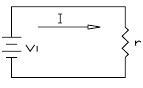
\includegraphics{image/fuente-tension}
\end{figure}

Para calcularla utilizaremos la ley de Ohn siguiente, $R=V/I$

\begin{itemize}
	\item Para el primer caso $R_{m}=5V/1A \rightarrow 5\Omega$
	\item Para el segundo caso $R_{m}=15V/0,5A \rightarrow 30 \Omega$
\end{itemize}

La resistencia mínima para $1A$ con $5V$ es $5\Omega$ y la resistencia mínima para $0.5A$ con $15V$ es $30 \Omega$. \newline

No debemos utilizar una resistencia mas pequeña, debido a que la intensidad que circularía seria mayor de lo que es capaz de suministrar la fuente de tensión. Aunque en el laboratorio las fuentes utilizadas dejan de suministrar tensión en tal caso, por motivos de seguridad frente a cortocircuitos y por ello no podemos verlo físicamente lo que sucede de verdad. \newline

\subsubsection{Medida de tensiones} 

\textit{Se utiliza un polímetro en la función de voltímetro. Para obtener la caída de tensión entre dos puntos de un circuito, basta colocar los dos terminales del voltímetro en los dos puntos del circuito. El voltímetro presenta una resistencia interna R, que al colocar en paralelo sobre los elementos del circuito, hace que el funcionamiento del circuito cambie. \newline
¿Cómo debe ser esta resistencia R, para que el circuito no sea modificado por el voltímetro?} 

\begin{figure}[h]
	\centering
	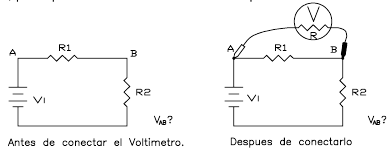
\includegraphics{image/medida-tension}
\end{figure}

Para ello el valor de la resistencia interna del voltímetro (RV) tiene que ser lo mayor posible ya que así, a la hora de conectar el voltímetro y formar parte del circuito, este no afectara al circuito ya que no pasara corriente por esta nueva rama y ira toda por el circuito que teníamos antes de conectar el voltímetro. \newline

\subsubsection{Medida de intensidad} 

\textit{Se utiliza un polímetro en función de amperímetro. Este aparato se debe conectar SIEMPRE en serie con aquella rama del circuito en la que se quiere conocer la intensidad (en caso de duda consultar al profesor). Entre los dos terminales, el amperímetro puede representarse como una resistencia, ésta modifica el circuito al realizar la medida.
¿Cómo debe ser la resistencia r, para que el circuito se modifique lo menos posible?}

\begin{figure}[h]
	\centering
	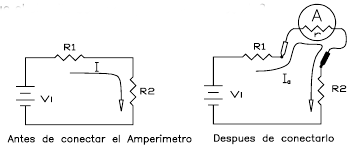
\includegraphics{image/medida-intensidad1}
\end{figure}

La que nos conviene, para que el circuito se modifique lo menos posible es, el menor valor posible ya que el medidor esta en serie y lo que necesitamos medir es la suma de todas las resistencias, cuanto menor sea el total de esta suma menor sera la intensidad afectada. \newline

\textit{Si el fabricante advierte que el amperímetro no puede soportar corrientes mayores que 0,2A: ¿Qué ocurre si se desea medir la corriente que circula por el circuito anterior, y por error, se hace como en la siguiente figura?  ¡No lo hagáis!  Es una cuestión teórica.} \newline

Se provocaría un cortocircuito con la batería del amperímetro debido a que tiene una resistencia muy baja y pasaría demasiada intensidad. \newline

\textit{¿Qué corriente circularía por el amperímetro?}

\begin{figure}[h]
	\centering
	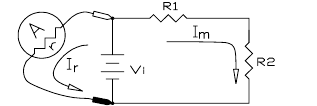
\includegraphics{image/medida-intensidad2}
\end{figure}

Teniendo en cuenta la ley de Ohm y que: $R_{1}=R_{2}=1k\Omega$ y $r =5\Omega V_{i}=5V$ \newline
$I=V/R \rightarrow 5V/5\Omega=1A$, entonces la corriente que circula por el amperímetro es de $1A$ y como es mayor que $0,2$ el fusible se romperá. \newline

\subsubsection{Medida de resistencias} 

\textit{Se utiliza un polímetro en la función de óhmetro. Se colocan en paralelo los dos terminales del polímetro sobre los extremos de la resistencia o agrupación de ellas que se desee medir. Nunca se deben medir resistencias cuando formen parte de un circuito, desconectar siempre la agrupación del resto del circuito. ¿Por qué debe hacerse así?} \newline

Porque si la resistencia no es desconectada, circulara corriente por ella, y esto genera lecturas erróneas. \newpage

\subsection{Resistencias y medidas en continua}

\subsubsection{Valor nominal y valor medido.} 

\textit{Coger 6 resistencias y crear una tabla con los valores medidos de las resistencias. Compararlos con con el valor nominal dado por el código de colores y comprobar que los valores medidos están dentro de la tolerancia especificada por el fabricante.} \newline

\subsubsection{Agrupación de resistencias. Medidas en un circuito} 

Se ha de montar la agrupación de 6 resistencias (parte derecha de la figura).
\begin{figure}[h]
	\centering
	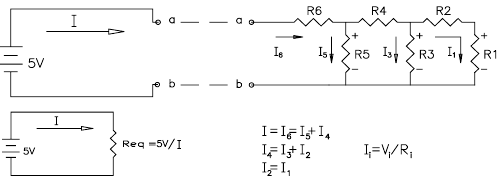
\includegraphics[scale=1]{image/agrupacion-resistencia}
\end{figure}

\begin{figure}[h]
	\centering
	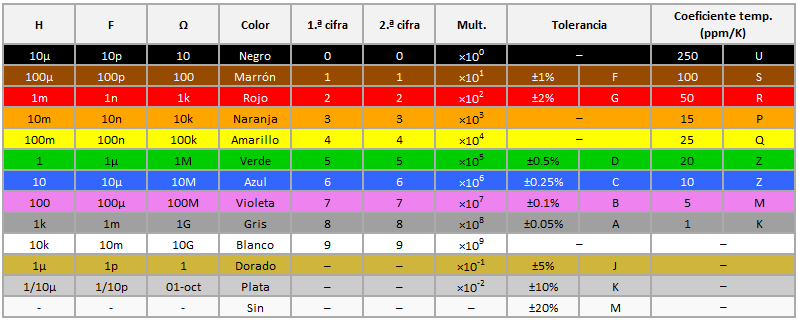
\includegraphics[scale=0.5]{image/valor-resistencia}
		\caption{Valores de las resistencias.} \label{Color-resistencia}
\end{figure}

\newpage

\textit{Calcular teóricamente (con los valores medidos de las resistencias) el valor de la agrupación. Medir con el polímetro la resistencia equivalente de la agrupación de resistencias.} 

\begin{figure}[h]
	\centering
	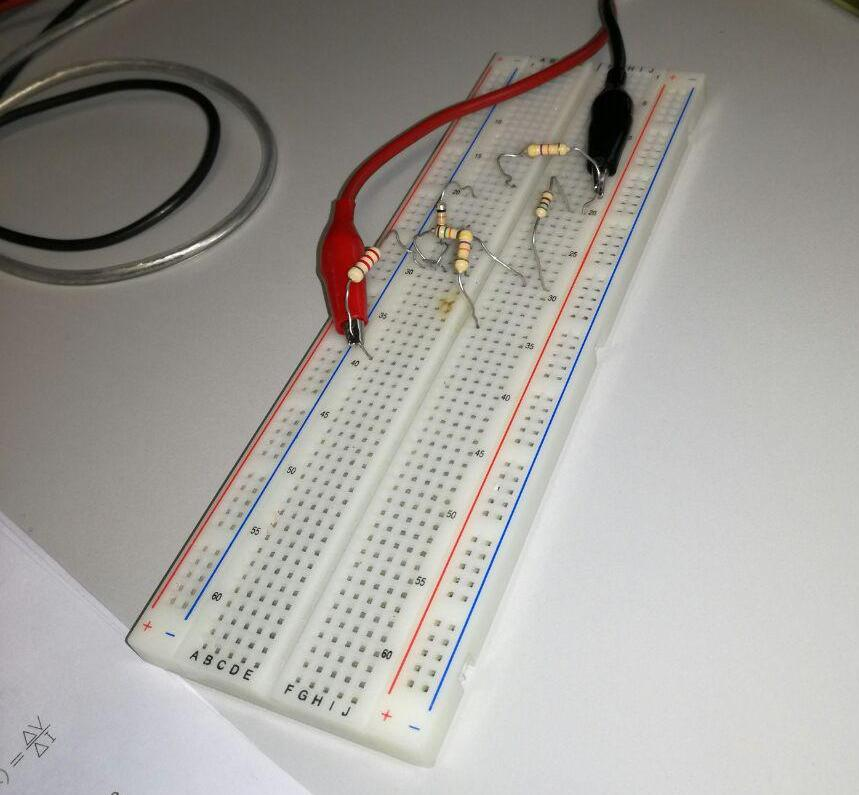
\includegraphics[scale=0.4]{image/practica1-resistencias2}
	\caption{Fotografía resistencias.} \label{Color-resistencia}
\end{figure}

\begin{table}[H]
	\centering
	\begin{tabular}[scale 0.3]{|c|c|c|c|c|}
		\hline
		\textbf{ID} & \textbf{COLOR} & \textbf{V.
			 NOMINAL} & \textbf{TOLERANCIA} & \textbf{V. MEDIDO} \\
		\hline
		$ R_{1} $ & Marrón, negro, naranja, oro & $10 K \Omega _{-}^{+}5 \% $ & $_{-}^{+}500 \Omega $ & $9.77K \Omega $ \\
		$ R_{2} $ & Marrón, negro, naranja, oro & $10 K \Omega _{-}^{+}5 \% $ & $_{-}^{+}500 \Omega $ & $9.69K \Omega $ \\
		$ R_{3} $ & Marrón, verde, naranja, oro & $15 K \Omega _{-}^{+}5 \% $ & $_{-}^{+}750 \Omega $ & $14.84K \Omega $ \\
		$ R_{4} $ & Naranja, negro, naranja, oro & $30 K \Omega _{-}^{+}5 \% $ & $_{-}^{+}1500 \Omega $ & $29.67K \Omega $ \\
		$ R_{5} $ & Amarillo, naranja, naranja, oro & $46 K \Omega _{-}^{+}5 \% $ & $_{-}^{+}2300 \Omega $ & $47.8K \Omega $\\	
		$ R_{6} $ & Marrón, negro, rojo, oro & $100 K \Omega _{-}^{+}5 \% $ & $_{-}^{+}50 \Omega $ & $98.1K \Omega $\\	
		\hline
	\end{tabular}  
	\caption{Valores de las resistencias obtenidas.} \label{Resistencias}
\end{table}

$ R_{A} = R_{1 \rightarrow 2} = R_{1} + R_{2} = 9.77K \Omega + 9.69K \Omega = 19.46K \Omega $ \newline

$ R_{B} = R_{A \rightarrow 3} = \dfrac{ R_{3} * R_{A} }{ { R_{3} + R_{A} } } = \dfrac{14.84K \Omega * 19.46K \Omega}{14.84K \Omega + 19.46K \Omega} = \dfrac{304.0156K \Omega}{34.3K \Omega} = 8.8634K \Omega $ \newline

$ R_{C} = R_{B \rightarrow 4} = R_{B} + R_{3} = 29.67K \Omega + 8.8634K \Omega = 38.5334K \Omega $ \newline

$ R_{B} = R_{C \rightarrow 5} = \dfrac{ R_{3} * R_{C} }{ { R_{3} + R_{C} } } = \dfrac{47.8K \Omega * 38.5334K \Omega}{47.8K \Omega + 38.5334K \Omega} = \dfrac{1841.8965K \Omega}{86.3334K \Omega} = 8.8634K \Omega $ \newline

$ R_{Equivalente} = R_{D \rightarrow 6} = R_{D} + R_{6} = 21.3347K \Omega + 98.1K \Omega = 21432.1K \Omega $ \newline

Por lo tanto la resistencia equivalente resultante teóricamente seria de $21432.1K \Omega$. \newline

\textit{Posteriormente, a la agrupación se le conecta una fuente de tensión de continua (en la figura aparece de 5V, pero puede ser de otro valor). Medir la intensidad que entra a la agrupación de resistencias (I en la figura). La resistencia equivalente será el cociente de 5V y la intensidad medida I (Req=5V/I).} \newline

$I=1.62mA$ \newline

$R_{eq} = \dfrac{5V}{1.62mA} = 3.0864 k \Omega$ \newline

\textit{Medir la diferencia de potencial en las resistencias $ R_{1} $, $ R_{3} $ y $ R_{5} $  ($VR_{1}$, $VR_{3}$ y $VR_{5}$). Medir la intensidad $ I_{1} $ Si es imposible medirla con los amperímetros del laboratorio, por ser muy pequeña, se debe medir la tensión en $ R_{1} $ (o $ R_{2} $) y dividir por $ R_{1} $ (o$  R_{2} $). Comprobar teóricamente que los resultados de $ VR_{1} $, $ VR_{3} $, $VR_{5} $ e $ I_{1} $ son correctos.} \newline

$VR_{1} = 0.673V$ \newline
$VR_{3} = 4.62V$ \newline
$VR_{5} = 5.68V$ \newline

$I_{1} = 1.46A$ \newpage

\subsubsection{Cálculo del coeficiente de variación de resistencia con la temperatura ($ \alpha $).} 

\textit{Sabemos que el valor de una resistencia cambia con la temperatura. Una fórmula aproximada que describe dicha variación es $ R(T)=R(T_{0})*[1 + \alpha (T $ - $ T_{0})] $. Esta fórmula la vamos a utilizar para calcular el coeficiente de temperatura ($ \alpha $) para el wolframio (el metal del filamento de las bombillas).} \newline

\textit{Primero se mide con el polímetro la resistencia $ R(T_{0}) $ de una bombilla T4W a temperatura ambiente (suponer $ T_{0}=295,15 K $, que corresponde a 22ºC). Luego se conecta la bombilla a 12 V, se mide la tensión V, y se mide la intensidad entrante con un amperímetro como en la figura, o mejor aún, tomar la corriente consumida de la pantalla de la propia fuente. El cociente $ V/I $ será el valor de $ R(T) $. Falta calcular la temperatura T, para eso utilizaremos la Ley de Stefan (ver recuadro). Si la temperatura T es mucho mayor que la temperatura ambiente (¡comprobarlo!) la potencia electromagnética radiada (P) es aproximadamente igual a la potencia eléctrica consumida por la bombilla (es decir $ P=I*V $). Tras haber calculado T, podemos despejar el valor del coeficiente de temperatura $ \alpha $.} \newline

\begin{figure}[h]
	\centering
	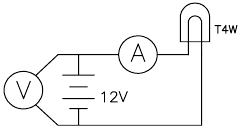
\includegraphics[scale=1]{image/bombilla}
\end{figure}

$ Bombilla \rightarrow 4W $ \newline

$ R_{Bombilla}=3.5 \Omega \rightarrow R_{Bombilla Caliente} = 3.89K \Omega $ \newline
$I_{Bombilla} = 0.32A $ \newline
$V_{Bombilla}=12.04V$ \newline

$R_{Caliente} = \dfrac{12.04V}{0.32A} = 37.625 \Omega $ \newline

$P_{Consumida}=I*V=3.3712 \omega $ \newline
$P_{Radiada}=eoAT^4 \rightarrow T$ \newline

$P_{Radiada}=eoAT^4 \rightarrow 3.3712 \omega = 1* 5.6704 * 10^-8 * 2.6 * 10^6 * T^4 \rightarrow T=2186.74 k$ \newline

$R_{t} = R(T_{0}) * [1+ \alpha (T - T_{0})] \rightarrow 37.625 \Omega = 3.5 \Omega + 6998.883=0.005615K^-1 $ \newpage

\textit{Comparar el valor obtenido de $\alpha$ con el proporcionado por otra fuente (libros, internet, etc.). Citar la fuente.} \newline

Le correspondería la luz infrarroja, fuente wikipedia. \newline

\textit{Calcular la longitud de onda $ \lambda MAX $ a la cual, la bombilla emite la máxima radiación. Utilizar la Ley del desplazamiento de Wien (ver recuadro). ¿A qué color corresponde $ \lambda MAX $?} \newline

$ \lambda MAX \; * \; T=2897768.5 $ \newline

$ \lambda MAX= \dfrac {2897768.5nmk}{2186.74k} =  1325.1545nm$ \newline

\newpage


\section{PRACTICA 01. Manejo del polímetro. Medidas en continua \cite{IV}} 

\subsection{Cuestiones teóricas}

\subsubsection{Fuente de Tensión} 

\textit{Una fuente de tensión ideal es un elemento que proporciona una tensión fija entre sus dos terminales. En el laboratorio se disponen de fuentes de +15V, -15V y +5V. Estas fuentes tienen una limitación de corriente de 0,5 y 1A; si se superan estos valores, se pueden destruir componentes de la fuente.} \newline

\textit{Calcular la resistencia mínima que se puede colocar en los extremos de la fuente de tensión, para que la corriente I que circula por el circuito sea menor que 1A (para Vi=5V) o menor que 0,5A (para Vi=15V). ¿Por qué no se debe utilizar una resistencia menor que la calculada?} \newline

\begin{figure}[h]
	\centering
	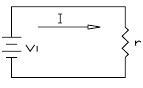
\includegraphics{image/fuente-tension}
\end{figure}

Para calcularla utilizaremos la ley de Ohn siguiente, $R=V/I$

\begin{itemize}
	\item Para el primer caso $R_{m}=5V/1A \rightarrow 5\Omega$ como mínimo
	\item Para el segundo caso $R_{m}=15V/0,5A \rightarrow 30 \Omega$ como mínimo
\end{itemize}

Si las resistencias fuesen menor que las calculadas con dichos voltajes, podríamos poner en peligro los elementos de la fuente ya que superaríamos las intensidades permitidas por la fuente de alimentación. \newline

\subsubsection{Medida de tensiones} 

\textit{Se utiliza un polímetro en la función de voltímetro. Para obtener la caída de tensión entre dos puntos de un circuito, basta colocar los dos terminales del voltímetro en los dos puntos del circuito. El voltímetro presenta una resistencia interna R, que al colocar en paralelo sobre los elementos del circuito, hace que el funcionamiento del circuito cambie. \newline
¿Cómo debe ser esta resistencia R, para que el circuito no sea modificado por el voltímetro?} 

\begin{figure}[H]
	\centering
	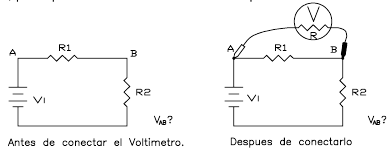
\includegraphics{image/medida-tension}
\end{figure}

Como el polímetro se conecta en paralelo, la suma de la resistencia del polímetro ( R ) y la resistencia del circuito ( R1 ) debe ser igual a R1. De esta forma no afectaríamos al circuito al conectar  el polímetro.

\subsubsection{Medida de intensidad} 

\textit{Se utiliza un polímetro en función de amperímetro. Este aparato se debe conectar SIEMPRE en serie con aquella rama del circuito en la que se quiere conocer la intensidad (en caso de duda consultar al profesor). Entre los dos terminales, el amperímetro puede representarse como una resistencia, ésta modifica el circuito al realizar la medida.
	¿Cómo debe ser la resistencia r, para que el circuito se modifique lo menos posible?}

\begin{figure}[h]
	\centering
	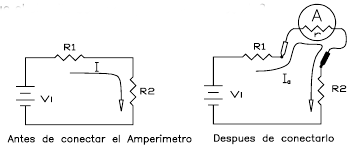
\includegraphics{image/medida-intensidad1}
\end{figure}

\newpage

Para que el circuito anterior se modifique lo menos posible al conectarle el polímetro, la resistencia r debe ser lo más pequeña posible ya que esta conectado en serie y: \newline

Rtotal =  R1 + R2+r con el polímetro

Rtotal = R1 + R2 sin el polímetro \newline

\textit{Si el fabricante advierte que el amperímetro no puede soportar corrientes mayores que 0,2A: ¿Qué ocurre si se desea medir la corriente que circula por el circuito anterior, y por error, se hace como en la siguiente figura?  ¡No lo hagáis!  Es una cuestión teórica.} \newline

Si se mide la corriente como en la figura anterior, la intensidad circularía directamente por el polímetro y no pasaría por el circuito con R1 y R2. \newline

Con lo cual estaríamos midiendo la intensidad que sale directamente de la fuente de alimentación \newline

\textit{¿Qué corriente circularía por el amperímetro?}

\begin{figure}[h]
	\centering
	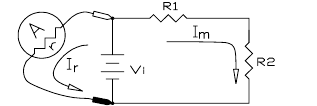
\includegraphics{image/medida-intensidad2}
\end{figure}

Como el amperímetro solo soporta corrientes <= 0,2 A si medimos la intensidad como en la figura anterior, estaría pasando una intensidad de: por la ley de Ohm I= V/R = 5/5 = 1 A, corriente mucho mayor que el límite del fabricante. Podríamos romper el amperímetro.\newline

\subsubsection{Medida de resistencias} 

\textit{Se utiliza un polímetro en la función de óhmetro. Se colocan en paralelo los dos terminales del polímetro sobre los extremos de la resistencia o agrupación de ellas que se desee medir. Nunca se deben medir resistencias cuando formen parte de un circuito, desconectar siempre la agrupación del resto del circuito. ¿Por qué debe hacerse así?} \newline

Porque el valor de la resistencia puede verse alterado por otros componentes del circuito. \newline

\subsection{Resistencias y medidas en continua}

\subsubsection{Valor nominal y valor medido.} 

\textit{Coger 6 resistencias y crear una tabla con los valores medidos de las resistencias. Compararlos con con el valor nominal dado por el código de colores y comprobar que los valores medidos están dentro de la tolerancia especificada por el fabricante.} \newline

\subsubsection{Agrupación de resistencias. Medidas en un circuito \cite{IA}.} 

Se ha de montar la agrupación de 6 resistencias (parte derecha de la figura).
\begin{figure}[h]
	\centering
	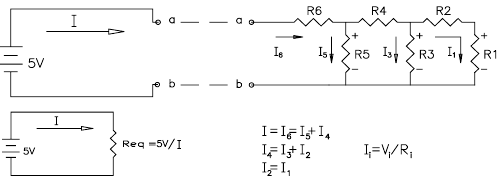
\includegraphics[scale=1]{image/agrupacion-resistencia}
\end{figure}

\textit{Calcular teóricamente (con los valores medidos de las resistencias) el valor de la agrupación. Medir con el polímetro la resistencia equivalente de la agrupación de resistencias.} \newline

\begin{figure}[H]
	\centering
	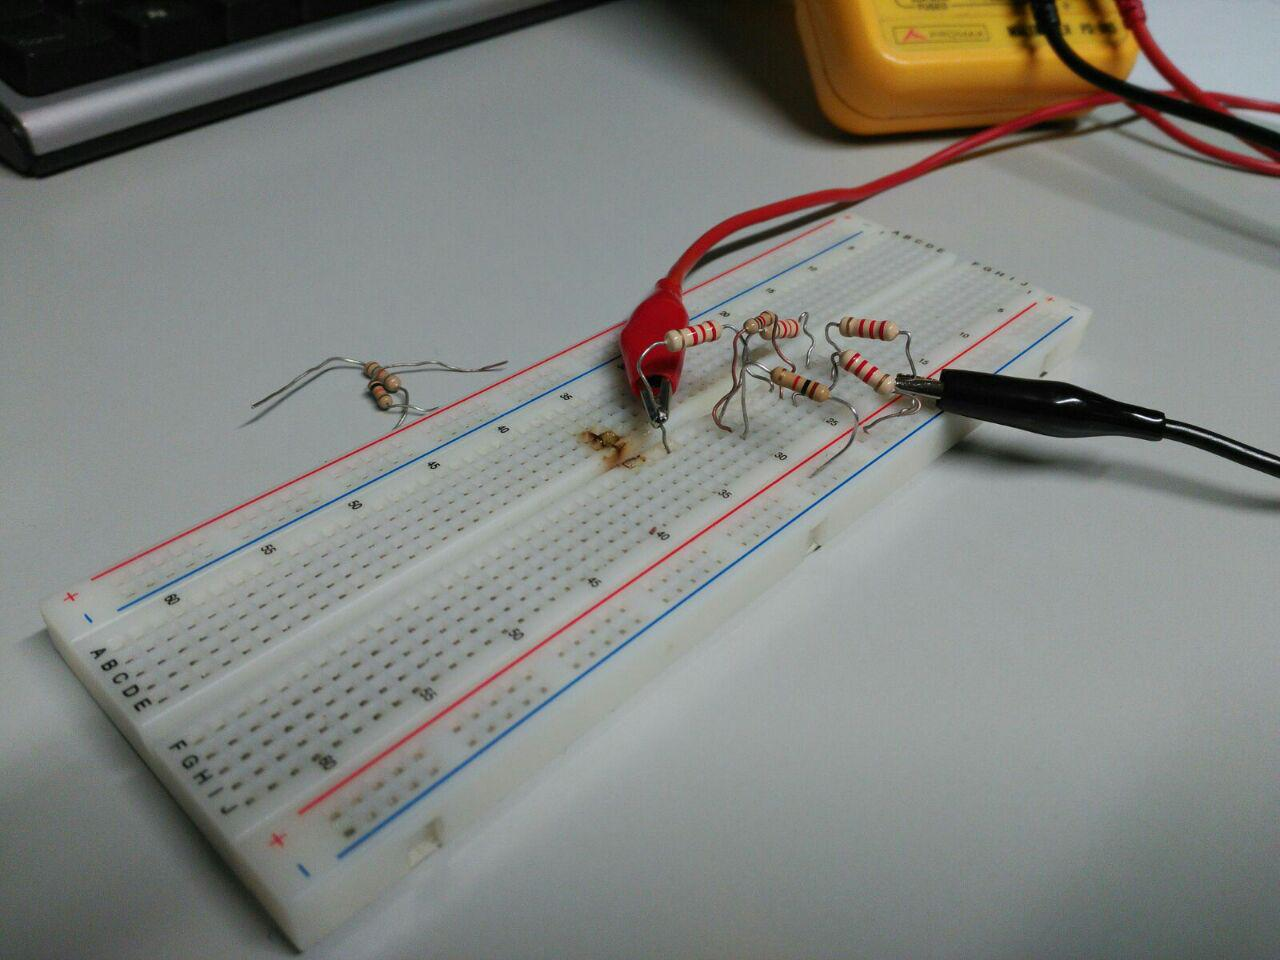
\includegraphics[scale=0.3]{image/practica1-resistencias}
	\caption{Fotografía resistencias.} \label{Color-resistencia}
\end{figure}

\begin{figure}[H]
	\centering
	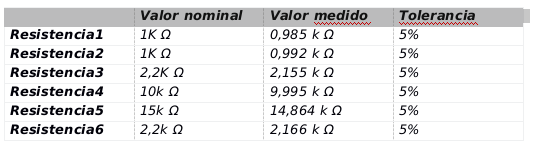
\includegraphics[width=\linewidth]{image/tablavictor}
	\label{fig:tablavictor}
\end{figure}


Calculando la suma de resistencias teóricamente: \newline
Agrupamos R1, R2, R4, R6 y las     sumamos normal ya que están en serie -> R1+R2+R4+R6 = $ 14,138 k \Omega $  y lo sumamos en paralelo con R3 y R5.  $(1/R3+1/R5+1/(R1+R2+R4+R6))^{-1} =  1,66 k \Omega $. \newline

Si lo comparamos con el valor medido en el laboratorio vemos que son muy similares. \newline

Valor medido: $ 1,64 k \Omega $. \newline

\textit{Posteriormente, a la agrupación se le conecta una fuente de tensión de continua (en la figura aparece de 5V, pero puede ser de otro valor). Medir la intensidad que entra a la agrupación de resistencias (I en la figura). La resistencia equivalente será el cociente de 5V y la intensidad medida I (Req=5V/I).} \newline

Si conectamos una fuente de alimentación de 5V, en la agrupación de resistencias entra una intensidad I1 = 0,91A.\newline

Por lo tanto, la resistencia equivalente tendría un valor de:$  5/0.91 = 5,49k \Omega $.

Si conectamos una fuente de alimentación de 15V, en la agrupación de resistencias entra una intensidad I1 = 2,78A.\newline

Por lo tanto, la resistencia equivalente tendría un valor de: $ 15/0.91 = 16.48k \Omega. $\newline

\textit{Medir la diferencia de potencial en las resistencias $ R_{1} $, $ R_{3} $ y $ R_{5} $  ($VR_{1}$, $VR_{3}$ y $VR_{5}$). Medir la intensidad $ I_{1} $ Si es imposible medirla con los amperímetros del laboratorio, por ser muy pequeña, se debe medir la tensión en $ R_{1} $ (o $ R_{2} $) y dividir por $ R_{1} $ (o$  R_{2} $). Comprobar teóricamente que los resultados de $ VR_{1} $, $ VR_{3} $, $VR_{5} $ e $ I_{1} $ son correctos.} \newline

La diferencia de potencial de R1 es de 0,36V. \newline

La diferencia de potencial de R3 es de 0,721V. \newline

La diferencia de potencial de R5 es de 1,22V.\newline

La intensidad medida I1, entrando 5V es de 0,91 A.\newline

\subsubsection{Cálculo del coeficiente de variación de resistencia con la temperatura ($ \alpha $).} 

\textit{Sabemos que el valor de una resistencia cambia con la temperatura. Una fórmula aproximada que describe dicha variación es $ R(T)=R(T_{0})*[1 + \alpha (T $ - $ T_{0})] $. Esta fórmula la vamos a utilizar para calcular el coeficiente de temperatura ($ \alpha $) para el wolframio (el metal del filamento de las bombillas).} \newline

\textit{Primero se mide con el polímetro la resistencia $ R(T_{0}) $ de una bombilla T4W a temperatura ambiente (suponer $ T_{0}=295,15 K $, que corresponde a 22ºC). Luego se conecta la bombilla a 12 V, se mide la tensión V, y se mide la intensidad entrante con un amperímetro como en la figura, o mejor aún, tomar la corriente consumida de la pantalla de la propia fuente. El cociente $ V/I $ será el valor de $ R(T) $. Falta calcular la temperatura T, para eso utilizaremos la Ley de Stefan (ver recuadro). Si la temperatura T es mucho mayor que la temperatura ambiente (¡comprobarlo!) la potencia electromagnética radiada (P) es aproximadamente igual a la potencia eléctrica consumida por la bombilla (es decir $ P=I*V $). Tras haber calculado T, podemos despejar el valor del coeficiente de temperatura $ \alpha $.} \newline

\begin{figure}[h]
	\centering
	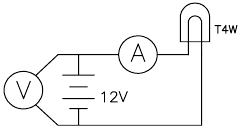
\includegraphics[scale=1]{image/bombilla}
\end{figure}

En primer lugar medimos la resistencia de la bombilla con el polímetro en frío (R(To)) y obtenemos un valor aproximado de $ R(To)=2.87 \Omega $.\newline

En segundo lugar medimos la intensidad que pasa por la bombilla al pasarle una tensión de 12V.Y obtenemos una I=0.35A. Con lo que podemos calcular utilizando la ley de Ohm la Resistencia (R(T)).\newline

Una vez tomadas las medidas, introducimos los datos en la fórmula de la ley de Stefan y calculamos la temperatura T. Como sabemos que e=1, la constante de Stefan-Boltzman tiene un valor de  $ [I=5,6704*10^{8} W/(m^{2}+K^{4})] $ y el área de la bombilla es aproximadamente $ 2,6*10-6m^{2} $ y que la P ( potencia ) es de 4W, podemos despejar la temperatura T. Haciendo los cálculos obtenemos un valor de la temperatura T=2282,276387 K.\newline

Utilizando que $ R(T)=R(T_{0})*[1+I(T - T_{0}) $, sustituyendo los valores mencionados anteriormente y sabiendo que $ T_{0}=295,15K $ despejamos $ \alpha $ y obtenemos un valor aproximado para el coeficiente de temperatura de $ \alpha =5,5085*10^{-3} $ .\newline

\textit{Comparar el valor obtenido de $\alpha$ con el proporcionado por otra fuente (libros, internet, etc.). Citar la fuente.} \newline

Hemos consultado una tabla de coeficientes de temperatura en internet y para el woframio el coeficiente de temperatura indicado es $ 4,5*10^{-3} $ lo cual esta en sintonía con el valor calculado ( con un error apreciable ). \newline

\textit{Calcular la longitud de onda $ \lambda MAX $ a la cual, la bombilla emite la máxima radiación. Utilizar la Ley del desplazamiento de Wien (ver recuadro). ¿A qué color corresponde $ \lambda MAX $?} \newline

Utilizando la ley de desplazamiento de Wien y suponiendo que la potencia máxima radiada por la bombilla es de 4W. Podemos calcular $ \lambda max $ y obtenemos un valor de:$ \lambda max =1269,347 nm $.\newline


Consultando el espectro de luz visible observamos que le correspondería a la luz infraroja. \newline

\newpage


%----------------------------------------------------------------------------------------
%	Pracitica 2
%----------------------------------------------------------------------------------------




\section{PRACTICA 02. Alterna. Amplificador operacional. Diagrama de Bode. \cite{IA}}

\subsection{Medidas en alterna}

\textit{Medir con el osciloscopio la amplitud, periodo y frecuencia de dos señales generadas por el oscilador. Una debe ser triangular, y la otra cuadrada, sus amplitudes y frecuencias deben ser distintas.} \newline
\textit{Se deben anotar las medidas (forma, amplitud, periodo, frecuencia) de las formas de onda que se han medido. En el osciloscopio digital, se pueden tomar medidas de tres formas distintas:}

\begin{itemize}
	\item \textit{midiendo divisiones y multiplicando por el factor de escala.}
	\item \textit{midiendo con los cursores.}
	\item \textit{dejando al osciloscopio que mida automáticamente (en ciertos casos la medida puede no ser válida).}
\end{itemize}

\textit{En el guión de prácticas debería aparecer una tabla con medidas, similar a la siguiente:} \newline



\begin{table}[H]
	\centering
	\begin{tabular}{|m{0.75cm}|m{3cm}|m{2.5cm}|m{2.5cm}|m{3cm}|m{2.5cm}|}
		\hline
			\multicolumn{3}{|c|}{\textbf{SEÑAL}} & \textbf{SENOIDAL} & \textbf{TRIANGULAR} & \textbf{CUADRADA} \\
		\hline
			\multicolumn{2}{|c|}{\textbf{FUENTE SEÑAL}} & \textbf{AMPLITUD PERIODO FRECUENCIA} & 4 Vpp \newline 500 s \newline 2 Khz & 10 Vpp \newline 100 s \newline 10 Khz & 8 Vpp \newline 250 s \newline 4 Khz \\
		\hline
			\multirow {3}{0.75cm}{\rotatebox{90}{\textbf{OSCILOSCOPIO}}} 
				& \textbf{DIVISORES} & \textbf{AMPLITUD PERIODO FRECUENCIA} & 4 Vpp \newline 500 s \newline 2 Khz & 10 Vpp \newline 100 s \newline 10 Khz & 8 Vpp	\newline 250 s \newline 4 Khz \\ \cline{2-6}
		
				& \textbf{CURSORES} & \textbf{AMPLITUD PERIODO FRECUENCIA} & 3,970 Vpp \newline 500 s\newline 2 Khz & 9,83 Vpp \newline 100 s \newline 10 Khz & 7,983 Vpp \newline 250 s \newline 4 Khz \\ \cline{2-6}
		 
				& \textbf{AUTOMÁTICO} & \textbf{AMPLITUD PERIODO FRECUENCIA} & 3,92 Vpp \newline 500 s \newline 2 Khz & 9,79 Vpp \newline 100 s \newline 10 Khz & 7,93 Vpp \newline 250 s \newline 4 Khz \\ \cline{2-6}
		\hline
	\end{tabular}
		\caption{Valores tomados en clase.} \label{medidas}
\end{table} \newpage

\subsection{Filtro con amplificador operacional. Diagrama de Bode}

\subsubsection{Filtro con amplificador operacional.}
\textit{Construir el filtro pasobaja (LP) que se muestra en la figura. La frecuencia de corte del filtro ($ f_{c} $)  deberá ser 2 kHz (la frecuencia será aproximada, en función del material disponible en el laboratorio). La ganancia de la etapa coincide con $ k=(1+R_{2}/R_{1})=2 $ (usar dos resistencias iguales).}

\begin{figure}[H]
	\centering
	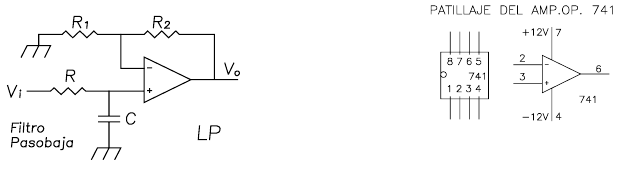
\includegraphics[scale=1]{image/filtro-baja}
\end{figure}

\begin{figure}[h]
	\centering
	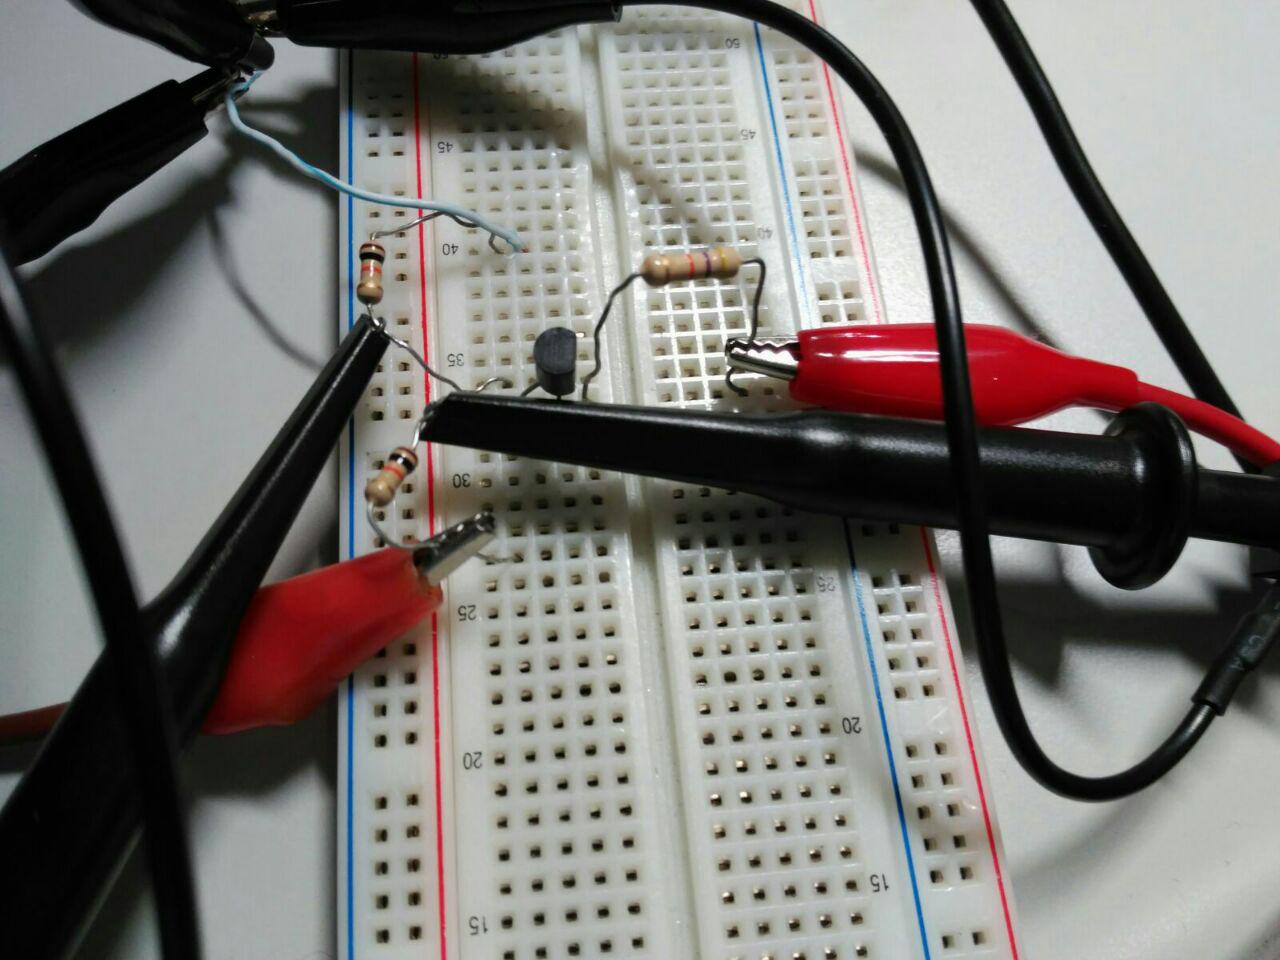
\includegraphics[scale=0.4]{image/practica3-A}
	\caption{Fotografía amplificador operacional.} \label{foto3a}
\end{figure}

\newpage

\textit{Indique los valores cogidos de R, C y $f_{c}$, y el proceso seguido para su elección.} \newline

$ R = 10 k \Omega $ \newline
$ C = 10 nF $ \newline
$ f_{c}=\dfrac{1}{(2 \pi * RC)} = \dfrac{1}{2 * \pi * 10 k \Omega * 10 nF} = 1592Hz$ \newline

\textit{Inmediatamente tras construir la etapa, debe comprobarse lo siguiente:}

\begin{itemize}
	\item \textit{La ganancia a bajas frecuencias en el pasobaja, debe ser igual a k=(1+R2/R1). Debería salir aproximadamente igual a 2 (6 dB).}
	\item \textit{La frecuencia de corte $ f_{c}=1/(2 \pi RC) $ está próxima a la teórica (según los valores de R y C escogidos). La frecuencia de corte es aquélla en la que la ganancia es $ \dfrac{k}{\sqrt{2}} =0,707k $ (caída de 3 dB). En nuestro caso, debería salir aproximadamente $ \dfrac{2}{\sqrt{2}}=1,4142 $ (3 dB, que es 6 dB menos la caída de 3 dB).}
	\item \textit{La ganancia a $ 10·fc $ en el filtro pasobaja debería salir aproximadamente igual a $ k/10=2/10=0,2 $ (-14 dB, que es 20 dB menos que la máxima ganancia de 6 dB).}
\end{itemize} \newpage

\subsubsection{Diagrama de Bode.}

\begin{itemize}
	\item Medir $ V_{i} $ y $ V_{o} $ desde 80 Hz hasta 50 kHz 
	\item Dar una tabla con las medidas de frecuencia, $ V_{i} $, $ V_{o} $, $ \dfrac{V_{o}}{V_{i}} $ y $ 20log(Vo/Vi) $.
	\item Hacer el diagrama de Bode en módulo. El diagrama de Bode tener al menos 20 puntos.
\end{itemize}

\begin{table}[H]
	\centering
	\begin{tabular}{|c|c|c|c|c|}
		\hline
			\textbf{f (Hz)} & \textbf{Vi(V)} & \textbf{V0(V)} & \textbf{V0/Vi (V)} & \textbf{20log(V0/Vi)} \\
		\hline 
			\textbf{80} &  10,3    & 10,2    & 0,990291262135922  &-0,084741058865094 \\
			\textbf{100} & 10,3    & 10,2    & 0,990291262135922  &-0,084741058865094 \\
			\textbf{200} & 10,3    & 10,2    & 0,990291262135922  &-0,084741058865094 \\
			\textbf{300} & 10,3    & 10,2    & 0,990291262135922  &-0,084741058865094 \\
			\textbf{500} & 10,3    & 9,7 & 0,941747572815534  &-0,521309808778548 \\
			\textbf{800} & 10,3    & 9,2 & 0,893203883495145  &-0,98098794719234 \\
			\textbf{1000} &    10,2    & 8,8 & 0,186274509803922  &-1,28234999223498 \\
			\textbf{1200} &    10,2    & 8,1 & 0,794117647058824  &-2,00230305766536 \\
			\textbf{1400} &    10,2    & 7,8 & 0,764705882352941  &-2,33011138142874 \\
			\textbf{1600} &    10,2    & 7,3 & 0,715686274509804  &-2,90554623282923 \\
			\textbf{1700} &    10,2    & 7,2 & 0,705882352941176  &-3,02535350661298 \\
			\textbf{1800} &    10,2    & 6,9 & 0,676470588235294  &-3,39502162049324 \\
			\textbf{2000} &    10,2    & 6,4 & 0,627450980392157  &-4,04840395556061 \\
			\textbf{3000} &    10,& 2    5   & 0,490196078431373  &-6,19260334851797 \\
			\textbf{5000} &    10,2    & 3,4 & 0,333333333333333  &-9,54242509439325 \\
			\textbf{8000} &    10,2    & 2,3 & 0,225490196078431  &-12,9374467148865 \\
			\textbf{10000} &   10,2    & 1,9 & 0,186274509803922  &-14,5969314161818 \\
			\textbf{20000} &   10,2    & 1,3 & 0,127450980392157  &-17,8931363891016 \\
			\textbf{30000} &   10,2    & 0,556   & 0,054509803921569  &-25,2705076035972 \\
			\textbf{50000} &   10  & 0,344   & 0,0344 &-29,2688311485694 \\
			\textbf{80000} &   10  & 0,231   & 0,0231 &-32,7277604021571 \\
			\textbf{100000} &  10  & 0,188   & 0,0188 &-34,5168430147264 \\
			\textbf{200000} &  10  & 0,106   & 0,0106 &-39,4938826947046 \\
			\textbf{300000} &  10  & 0,075   & 0,0075 &-42,498774732166 \\
			\textbf{500000} &  9,8 & 0,056   & 0,005714285714286  &-44,8607609737259 \\
		\hline			
	\end{tabular}
	\caption{Valores del diagrama de Bode. \cite{IA}} \label{Bode}
\end{table}

\begin{figure}[H]
	\centering
	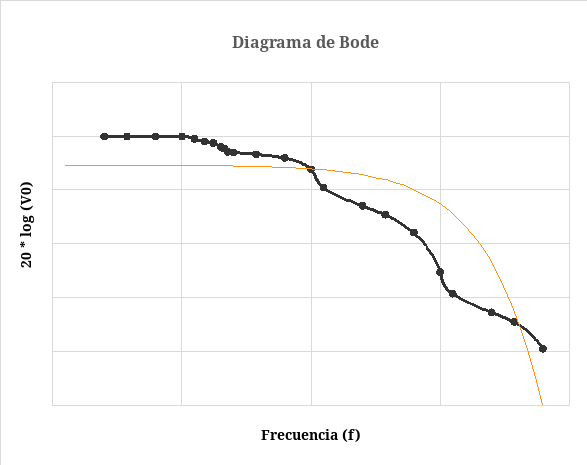
\includegraphics[scale=1]{image/diagrama-bode}
	\caption{Gráfica Bode \cite{IA}}
	\label{fig:diagrama-bode}
\end{figure}

\newpage

\section{PRACTICA 02. Alterna. Amplificador operacional. Diagrama de Bode. \cite{IV}}

\subsection{Medidas en alterna}

\textit{Medir con el osciloscopio la amplitud, periodo y frecuencia de dos señales generadas por el oscilador. Una debe ser triangular, y la otra cuadrada, sus amplitudes y frecuencias deben ser distintas.} \newline
\textit{Se deben anotar las medidas (forma, amplitud, periodo, frecuencia) de las formas de onda que se han medido. En el osciloscopio digital, se pueden tomar medidas de tres formas distintas:}

\begin{itemize}
	\item \textit{midiendo divisiones y multiplicando por el factor de escala.}
	\item \textit{midiendo con los cursores.}
	\item \textit{dejando al osciloscopio que mida automáticamente (en ciertos casos la medida puede no ser válida).}
\end{itemize}

\textit{En el guión de prácticas debería aparecer una tabla con medidas, similar a la siguiente:} \newline

\begin{figure}[H]
\centering
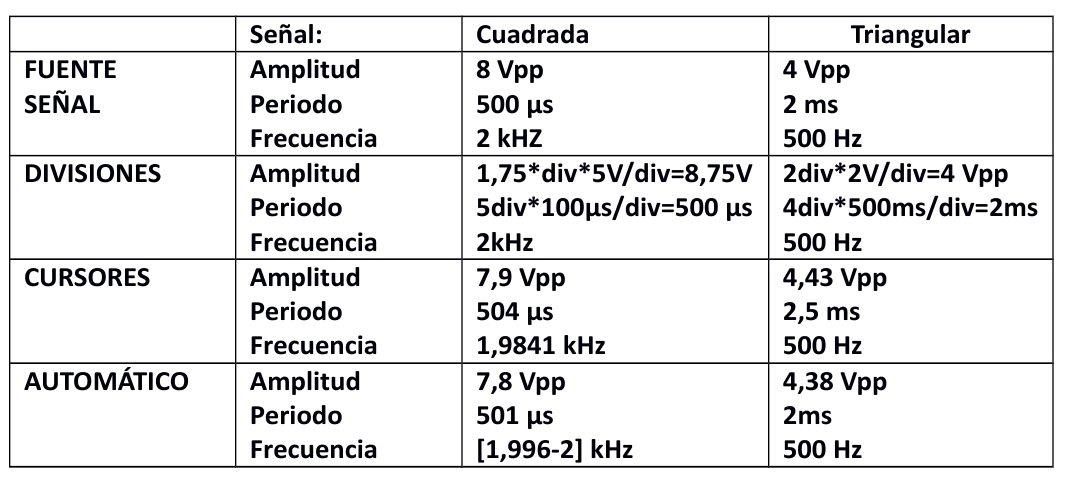
\includegraphics[width=1\linewidth]{image/tablavictor2}
\label{fig:tablavictor2}
\end{figure}


 \newpage

\subsection{Filtro con amplificador operacional. Diagrama de Bode}

\subsubsection{Filtro con amplificador operacional. \cite{IA}}
\textit{Construir el filtro pasobaja (LP) que se muestra en la figura. La frecuencia de corte del filtro ($ f_{c} $)  deberá ser 2 kHz (la frecuencia será aproximada, en función del material disponible en el laboratorio). La ganancia de la etapa coincide con $ k=(1+R_{2}/R_{1})=2 $ (usar dos resistencias iguales).}

\begin{figure}[H]
	\centering
	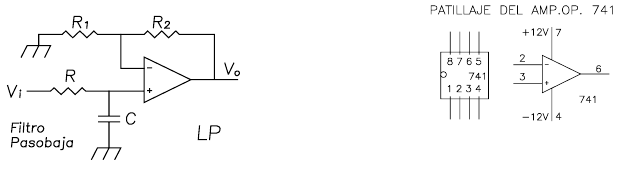
\includegraphics[scale=1]{image/filtro-baja}
\end{figure}

\begin{figure}[h]
	\centering
	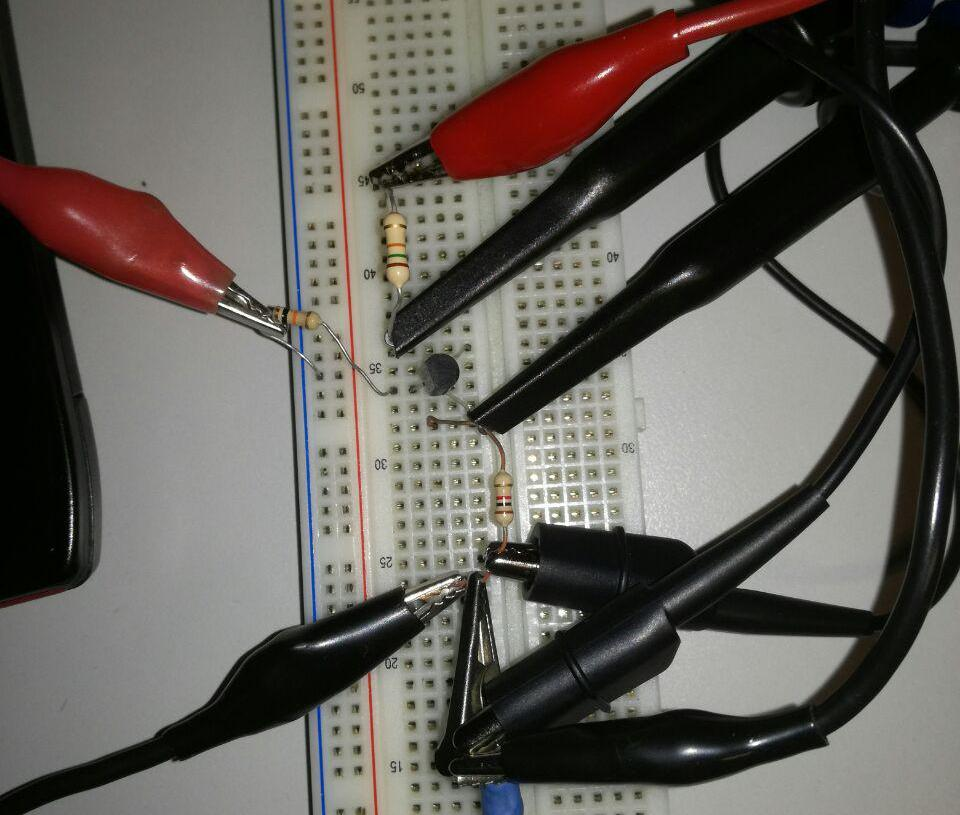
\includegraphics[scale=0.4]{image/ampli-victor}
	\caption{Fotografía amplificador operacional.} \label{foto3a}
\end{figure}

\newpage

\textit{Indique los valores cogidos de R, C y $f_{c}$, y el proceso seguido para su elección.} \newline

\textit{Inmediatamente tras construir la etapa, debe comprobarse lo siguiente:}

\begin{itemize}
	\item \textit{La ganancia a bajas frecuencias en el pasobaja, debe ser igual a k=(1+R2/R1). Debería salir aproximadamente igual a 2 (6 dB).}
	\item \textit{La frecuencia de corte $ f_{c}=1/(2 \pi RC) $ está próxima a la teórica (según los valores de R y C escogidos). La frecuencia de corte es aquélla en la que la ganancia es $ \dfrac{k}{\sqrt{2}} =0,707k $ (caída de 3 dB). En nuestro caso, debería salir aproximadamente $ \dfrac{2}{\sqrt{2}}=1,4142 $ (3 dB, que es 6 dB menos la caída de 3 dB).}
	\item \textit{La ganancia a $ 10·fc $ en el filtro paso baja debería salir aproximadamente igual a $ k/10=2/10=0,2 $ (-14 dB, que es 20 dB menos que la máxima ganancia de 6 dB).}
\end{itemize} 


Montamos el circuito con el material disponible en el laboratorio:\newline

R1 y R2 con un valor de $ 1k\Omega y R=15k\Omega $ . Disponemos de un amplificador operacional y de un condensador con $ C=2,2nF $. \newline

Medimos R1 y R2 con el polímetro y obtenemos:$  R1=0.985K\Omega  $  y  $ R2=0.992k \Omega $ \newline

Calculamos la ganancia $ k=1+R2/R1=2.0071 $. Con lo cual nos doblará la señal introducida.
\newline

A continuación calculamos la frecuencia de corte:\newline

Sustituimos nuestros datos donde $ R=15k\Omega $ y $ C=2.2nF $ y obtenemos \newline

Fc=4822.877063 Hz\newline


Con los datos tomados y calculando 20*log (Vi/Vo) en cada valor de la frecuéncia, obtenemos este gráfico por dispersión de la señal.\newline

\newpage



\subsubsection{Diagrama de Bode.}

\begin{itemize}
	\item Medir $ V_{i} $ y $ V_{o} $ desde 80 Hz hasta 50 kHz 
	\item Dar una tabla con las medidas de frecuencia, $ V_{i} $, $ V_{o} $, $ \dfrac{V_{o}}{V_{i}} $ y $ 20log(Vo/Vi) $.
	\item Hacer el diagrama de Bode en módulo. El diagrama de Bode tener al menos 20 puntos.
\end{itemize}

\begin{table}[H]
	\centering
	\begin{tabular}{|c|c|c|c|c|}
		\hline
		\textbf{Vi(V)} & \textbf{V0/Vi (V)} & \textbf{f (Hz)} & \textbf{20log(V0/Vi)} \\
		\hline 
		12,7&2,116666667&100&6,513049411\\
		12,7&2,116666667&200&6,513049411\\
		12,7&2,116666667&400&6,513049411\\
		12,7&2,116666667&500&6,513049411\\
		12,7&2,116666667&1000&6,513049411\\
		12,7&2,116666667&2000&6,513049411\\
		12,7&2,116666667&2500&6,513049411\\
		12,7&2,116666667&3000&6,513049411\\
		12,5&2,083333333&4000&6,375175252\\
		12,3&2,05&4100&6,235077221\\
		12,3&2,05&4200&6,235077221\\
		12,2&2,033333333&4300&6,164171606\\
		12,1&2,016666667&4500&6,092682399\\
		12&2&4600&6,020599913\\
		11,9&1,983333333&4700&5,94791422\\
		11,9&1,983333333&4800&5,94791422\\
		11,8&1,966666667&4900&5,874615138\\
		11,7&1,95&5000&5,800692227\\
		11,6&1,933333333&5500&5,726134777\\
		11,6&1,933333333&6000&5,726134777\\
		11,1&1,85&7000&5,343434568\\
		10,8&1,8&8000&5,105450102\\
		10&1,666666667&9000&4,436974992\\
		9,2&1,533333333&10000&3,712731539\\
		8,9&1,483333333&11000&3,424775125\\
		8,01&1,335&12000&2,509625314\\
		7,7&1,283333333&13000&2,166789496\\
		5,6&0,933333333&15000&-0,599264468\\
		4,5&0,75&20000&-2,498774732\\
		3,6&0,6&25000&-4,436974992\\
		3&0,5&30000&-6,020599913\\
		2,3&0,383333333&40000&-8,328468287\\
		2&0,333333333&50000&-9,542425094\\
		1,9&0,316666667&60000&-9,987952989\\
		1,3&0,216666667&100000&-13,28415796\\
	
		\hline			
	\end{tabular}
	\caption{Valores del diagrama de Bode.} \label{Bode}
\end{table}

\begin{figure}[H]
	\centering
	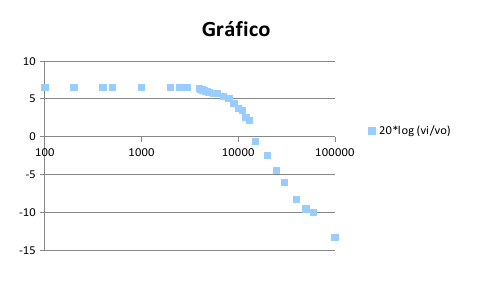
\includegraphics[scale=1.2]{image/bodevictor}
	\caption{Gráfica Bode}
	\label{fig:bodevictor}
\end{figure}


\newpage
%----------------------------------------------------------------------------------------
%	Pracitica 3
%----------------------------------------------------------------------------------------

\section{PRACTICA 03. Diodo. Unión PN \cite{2c}}

\subsection{Polarización directa. Tensión umbral ($ V_{\gamma} $) y resistencia dinámica ($ r_{d} $)}

\textit{Lo descrito en este apartado se hará con 3 ó 4 diodos, procurando que tengan una tensión umbral lo más distinta posible.} 

\begin{itemize}
	\item \textit{Medir la tensión umbral $ V_{\gamma} $ con el polímetro. Apuntar su valor en una tabla similar a la que aparece al final de este apartado.} 

	\item \textit{Montar el circuito de la figura. Se conecta en Vi el canal 1 del osciloscopio y en Vo el canal 2. Una onda triangular de frecuencia 1 kHz se conecta en Vi. La tensión de esta onda deberá variar entre 0 V y 5 V (6 V si $ V_{\gamma} $ es mayor que 1,5V) con resistencia $ R=120 \Omega $. Comprobar que en modo XY, en la pantalla se ve una aproximación de la curva I-V de un diodo.} 

	\begin{figure}[h]
	\centering
	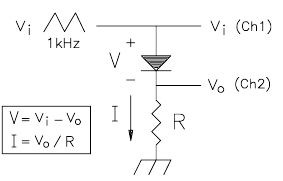
\includegraphics[width=0.4\linewidth]{image/screenshot002}
	\end{figure}

	\textit{Antes de capturar los datos con el osciloscopio, comprobar:} 
	\begin{itemize}
		\item \textit{El osciloscopio debe estar en [Acquire]-[Normal] para que no haga ningún tipo de media.}
		\item \textit{Los circuitos limitadores de ruido están encendidos en los dos canales. BW-Limit debe estar en ON.}
		\item \textit{La longitud del fichero CSV debe ser de 1.000 puntos.}
	\end{itemize}
	
	\item \textit{En el osciloscopio se debe medir la tensión umbral $ V_{\gamma} $ como se indica en la figura de la derecha, y se apunta en la columna correspondiente de la tabla.}

	\item \textit{Hacer una captura de los datos numéricos de los canales ¡en formato CSV! para cada diodo.}
	
	\item \textit{Posteriormente, en casa, y con una hoja de cálculo, se debe realizar una gráfica con los datos (CSV) de los diodos. (En la gráfica de muestra se han incluido más diodos de los necesarios.)}
	
	\begin{figure}[H]
	\centering
	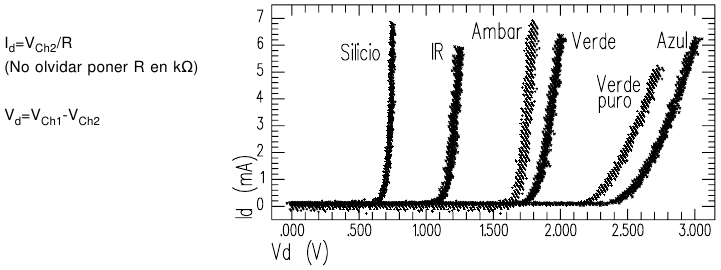
\includegraphics[width=0.7\linewidth]{image/screenshot003}
	\end{figure}

	\item \textit{Encontrar, para cada diodo, el valor máximo (aproximado) de $ I_{d} $ y $ V_{d} $. Con ellos, y $ V_{\gamma} $, se puede calcular la resistencia $ (r_{d} = (V_{d-max} - V_{ \gamma } )/I_{d-max} $. $ r_{d} $ debe estar en ohmios).}
	
	\begin{table}[H]
		\centering
		\begin{tabular}{|m{2.2cm}|m{2.2cm}|m{2.2cm}|m{2.2cm}|m{2.2cm}|m{2.2cm}|}
			\hline
			Diodo & $ V_{ \gamma } (V) $ \newline $ (polimetro) $ & $ V_{ \gamma } (V) $ \newline $ (osciloscopio) $ & $ V_{d-max} (V) $ & $ I_{d-max} (mA) $ & $ rd( \omega ) $ \\
			\hline
			verde & 1.7 & 2.1 & 5 & 3.127 & 0.319 \\
			\hline
			roja & 1.7 & 1.899 & 5 & 3.19 & 0.320 \\
			\hline
			negra & 0.698 & 0.822 & 5.1 & 4.39 & 0.205 \\
			\hline
		\end{tabular}
		\caption{Tabla que contiene los valores obtenidos en la practica 3}
		\label{fig:tabla-prac-4A2}
	\end{table}
	
	\begin{figure}[H]
		\centering
		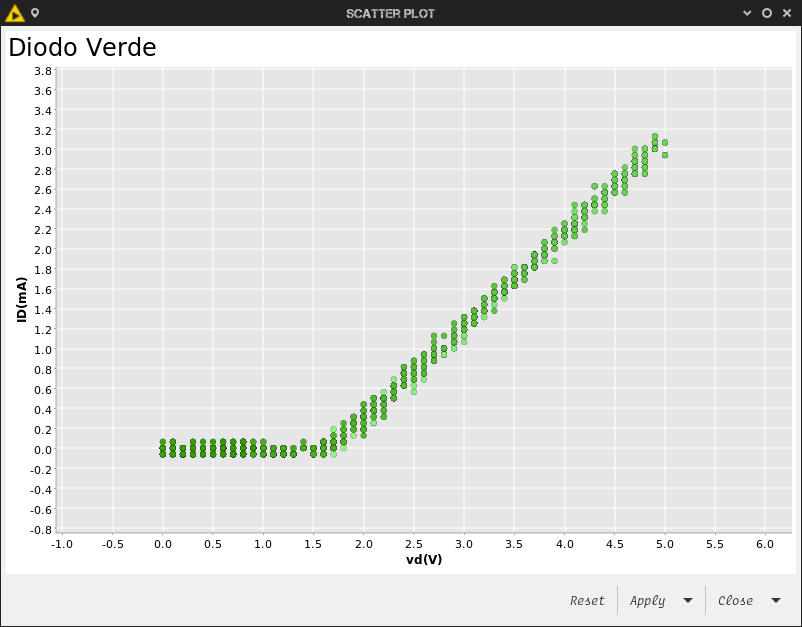
\includegraphics[scale=0.4]{image/diodo-verde}
		\caption{Gráfica diodo verde}
		\label{fig:grafica-diodo-verde}
	\end{figure}
	
	\begin{figure}[H]
		\centering
		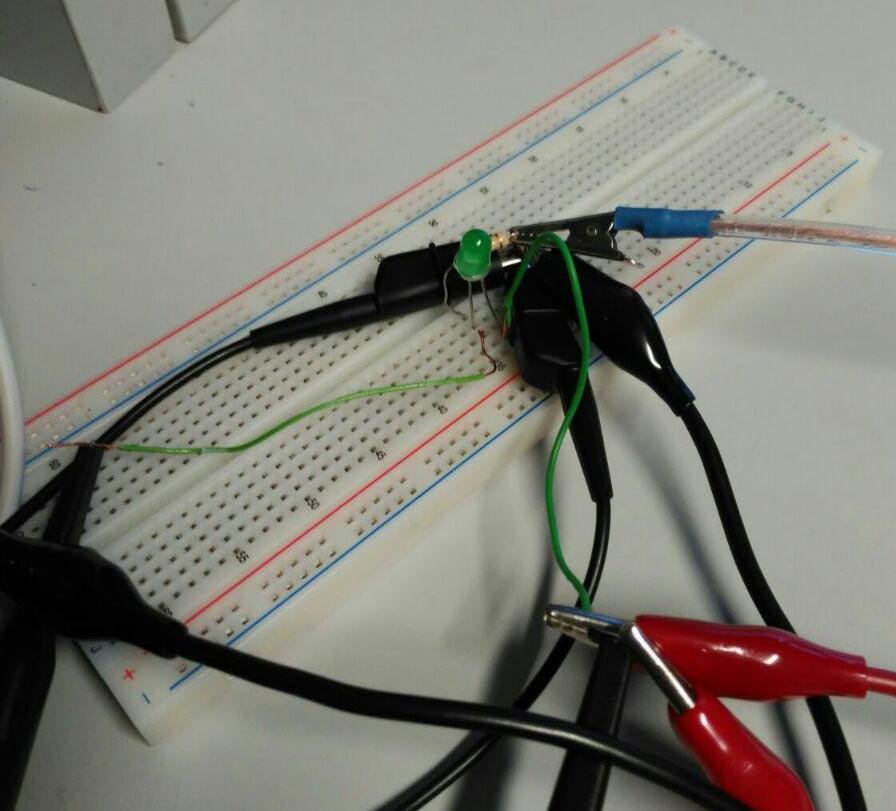
\includegraphics[scale=0.4]{image/foto-diodo-verde}
		\caption{Foto diodo verde}
		\label{fig:foto-diodo-verde}
	\end{figure}
	
	\begin{figure}[H]
		\centering
		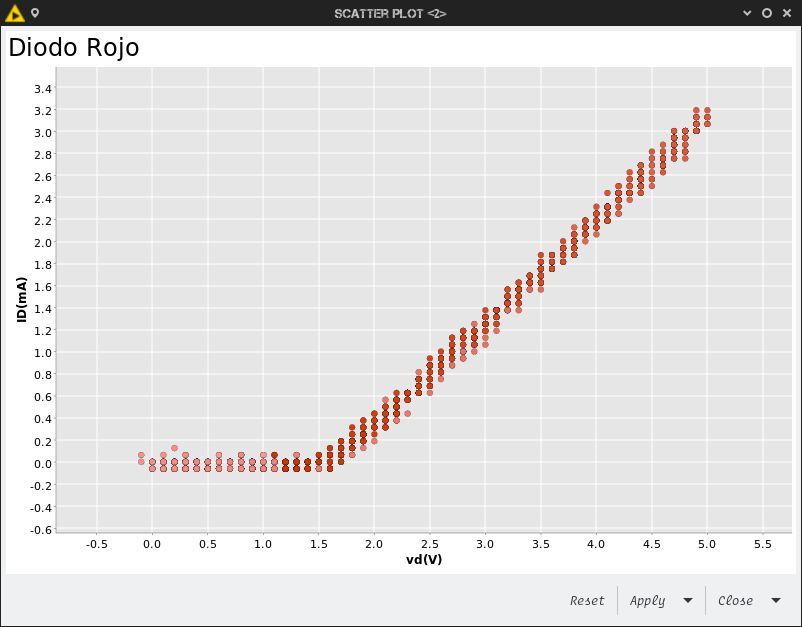
\includegraphics[scale=0.4]{image/diodo-rojo}
		\caption{Gráfica diodo rojo}
		\label{fig:grafica-diodo-rojo}
	\end{figure}
	
	\begin{figure}[H]
		\centering
		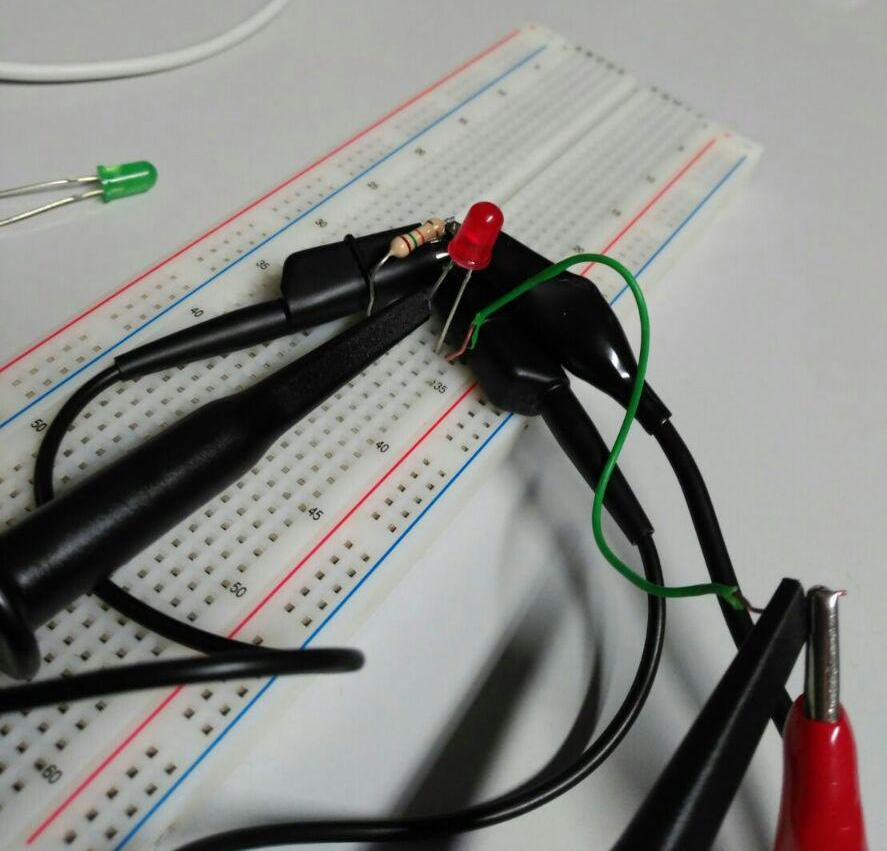
\includegraphics[scale=0.4]{image/foto-diodo-rojo}
		\caption{Foto diodo rojo}
		\label{fig:foto-diodo-rojo}
	\end{figure}
	
	\begin{figure}[H]
		\centering
		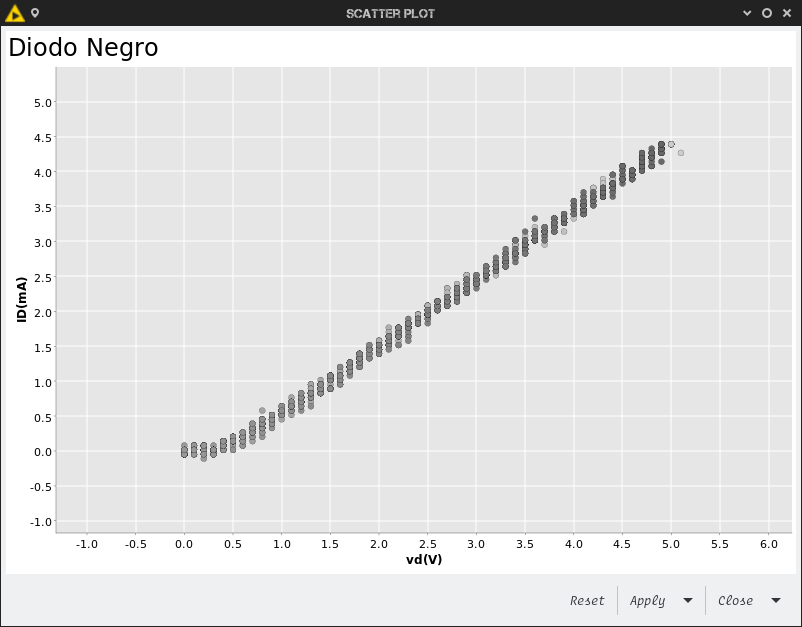
\includegraphics[scale=0.4]{image/diodo-negro}
		\caption{Gráfica diodo negro}
		\label{fig:grafica-diodo-negro}
	\end{figure}
	
	\begin{figure}[H]
		\centering
		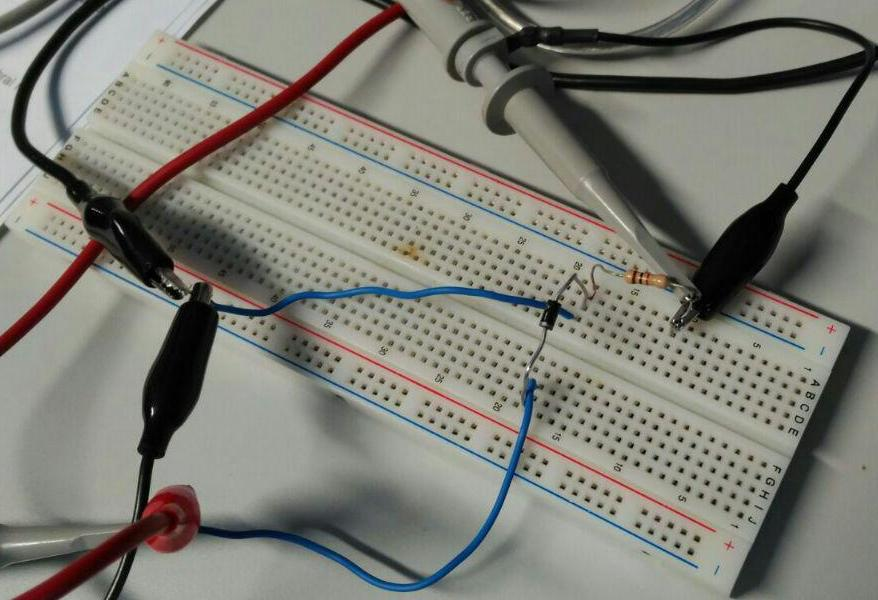
\includegraphics[scale=0.5]{image/foto-diodo-negro}
		\caption{Foto diodo negro}
		\label{fig:foto-diodo-negro}
	\end{figure}
	
	\begin{figure}[H]
		\centering
		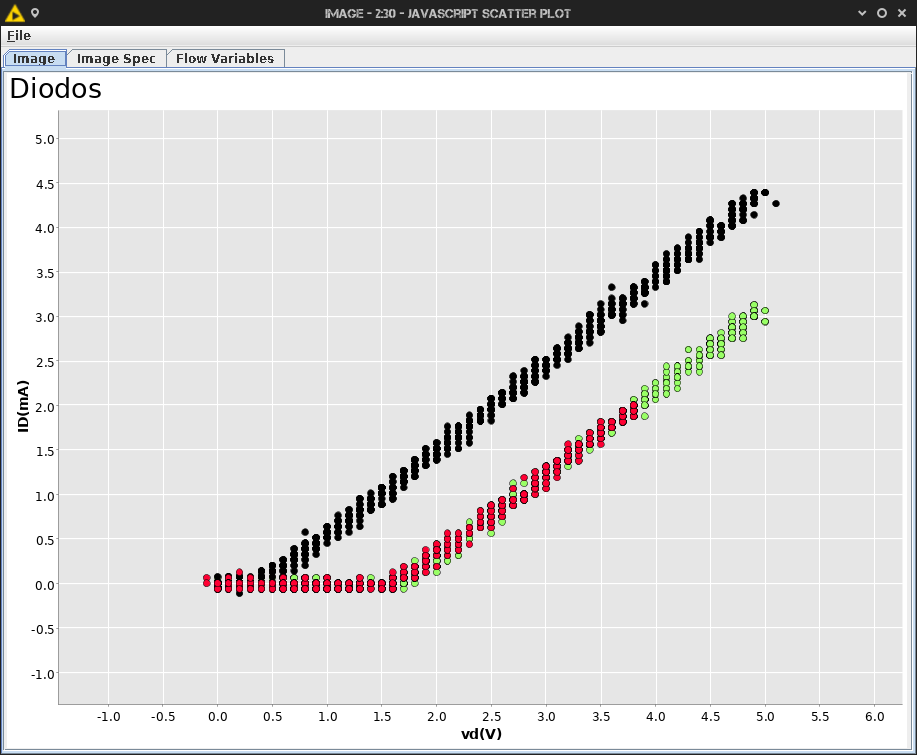
\includegraphics[scale=0.35]{image/all-diodos}
		\caption{Gráfica diodos juntos}
		\label{fig:grafica-diodo-todos}
	\end{figure}
	
\end{itemize}

\newpage

\subsection{Diodo sin polarización, funcionando como célula fotovoltaica}

\textit{Con un LED (preferentemente verde), montar el circuito de la figura, que no tiene polarización aplicada. Mida con el voltímetro la tensión VO, y verá que es mayor cuanto mayor sea la intensidad luminosa incidente en el LED. Parte de la potencia generada en el LED se pierde en el propio LED. A la máxima iluminación posible, calcule la potencia consumida en la resistencia (P= I·VO = VO2/R).} \newline

Para una resistencia de 46K$ \Omega $ y lo alumbramos con el voltímetro la caída de tensión y obtenemos:

\begin{figure}[H]
	\centering
	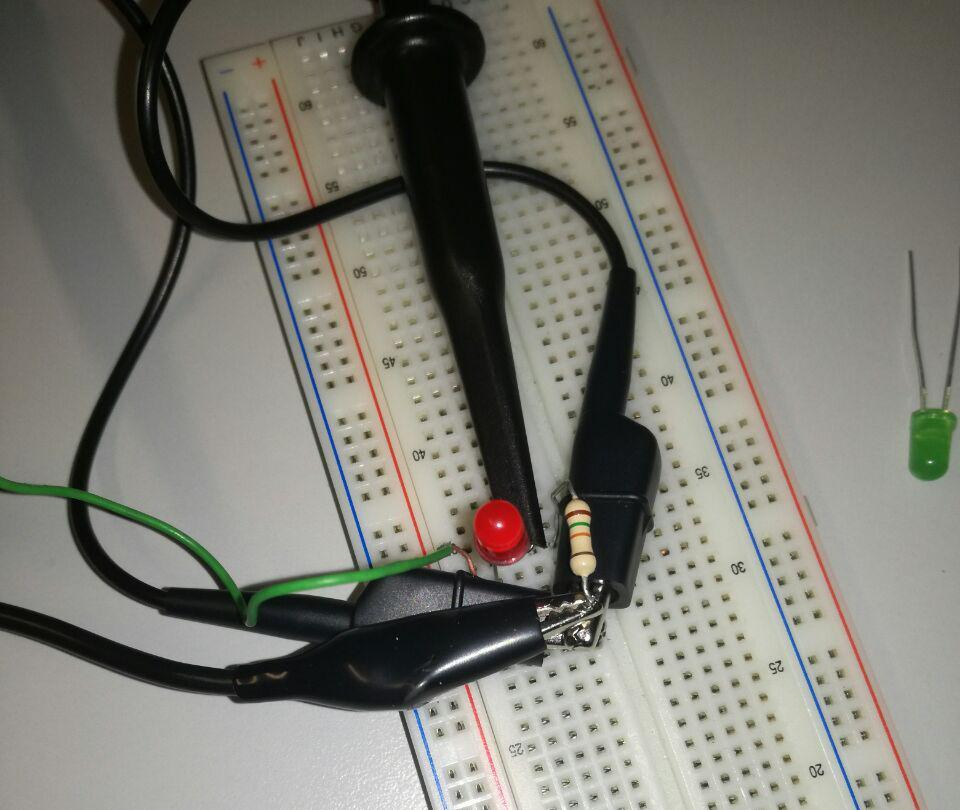
\includegraphics[scale=0.4]{image/lex-diodo}
	\caption{Foto luz diodo rojo}
	\label{fig:lex-diodo-rojo}
\end{figure}

\begin{table}[H]
	\centering
	\begin{tabular}{|c|c|}
		\hline
			Diodo & mV \\
		\hline
			Rojo & 8.32 \\
		\hline
	\end{tabular}
\end{table}

Por lo tanto la tensión consumida en la resistencia es de: \newline

$ P_{consumida} = V_{0}^{2} / R = 0.832V^{2} / 46000 \Omega = 1.5 * 10^{-5} \mu W $ \newline

\newpage

\textit{¿Cuántos LED serían necesarios para hacer funcionar una bombilla de 40W?} \newline

\begin{figure}[H]
	\centering
	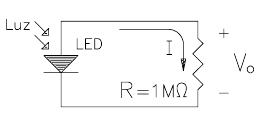
\includegraphics{image/screenshot005}
\end{figure}

$ 40 / (1.5 * 10^{-5}*10^{-6}) = 2.66 * 10^{12} $ , por lo tanto necesitamos $ 2.66 * 10^{12} $  para hacer funcionar una bombilla de 40W. \newline

\newpage

\section{PRACTICA 04. Tránsistor bipolar de union}

\subsection{Curva característica de salida (IC frente a VCE)  \cite{error1,2c}}

\textit{Con el polímetro, mida $ \beta $ ($ \beta _{F}$) del transistor que va a usarse en la práctica. Monte el circuito de la figura. $ V_{CC} $ es una onda triangular de 0 a 5V, y $ V_{i} $ es una tensión continua tomada de la fuente variable de continua. Conecte los canales 1 y 2 del osciloscopio tal como se indica en la figura.} \newline

$$ R_{B}=10K\Omega \hspace{2cm} R_{C}=47K\Omega \hspace{2cm} R_{E}=1K\Omega $$

\begin{figure}[H]
\centering
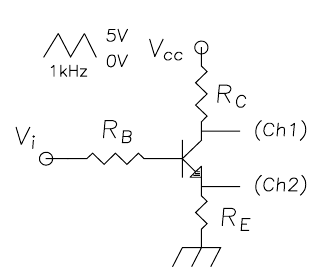
\includegraphics[width=0.4\linewidth]{image/p4f1}
\end{figure}

\begin{figure}[H]
	\centering
	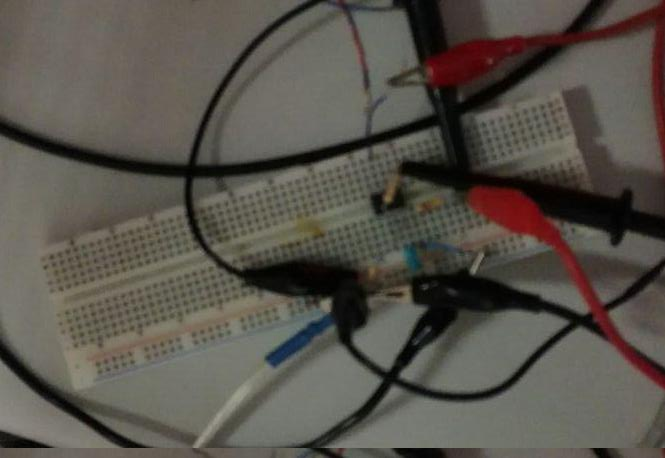
\includegraphics[scale=0.7]{image/transistorA}
	\caption{Fotografía transistor bipolar de unión}
	\label{fig:foto-transistorA}
\end{figure}

\textit{En el osciloscopio:}

\begin{itemize}
	\item \textit{Poner BW-limit=ON en Ch2 y Average=1 en [Acquire].}
	\item \textit{Hacer que la longitud del fichero CSV sea 500.}
	\item \textit{Poner modo XY, debería verse la curva característica.}
	\item \textit{Parar con Stop, no con Single, y grabar los datos en disquete con Quickprint.}
\end{itemize}

\textit{Debe entregarse una gráfica con 3 curvas (como la figura, pero ésta tiene más). Las 3 curvas corresponderán a tres tensiones $ V_{i} $ de valores comprendidos entre 0,8 y 6V. Debe completarse la tabla asociada: $ V_{i} $ valor tomado, $ V_{BE} $ medido con el polímetro, $ V_{E} $ (=$ V_{CH2} $) medido en ZAD con los cursores del osciloscopio, $ I_{E-osc} $ valor calculado como $ I_{E-osc}=V_{E}/R_{E} $, $ \beta_{osc} $ (calculado despejando $ \beta $ de la ecuación 1, y usando la $ I_{E-osc} $).} 

\textit{Calcule la media de $ \beta_{osc} $ y compárela con la $ \beta $ del polímetro. ¿Cuál es el error relativo del polímetro en la medida de $ \beta $?} \newline

$$ Ecuación 1: \; I_{E}=[ (V_{i}-V_{BE})/(R_{B}+(\beta +1)*R_{E}) ] (\beta +1) $$

\begin{figure}[H]
	\centering
	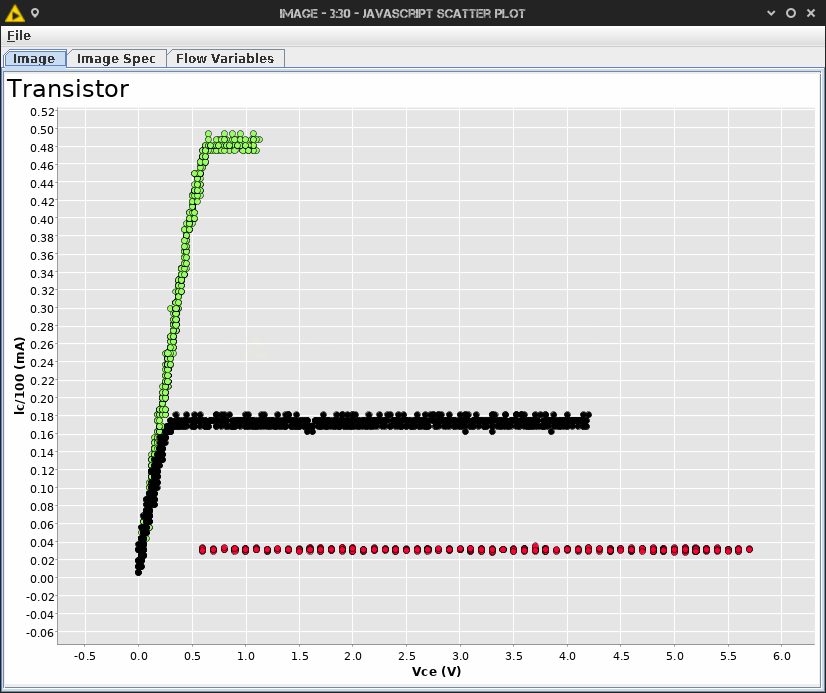
\includegraphics[scale=0.4]{image/transistor}
	\caption{Gráfica que contiene las tres curvas, correspondiente a las tres tensiones}
	\label{fig:Gráfica-prac-4A}
\end{figure}

Nos damos cuenta que la $ I_{E} $ es indiferente y menospreciamos el 0.13 porque las otras cifras son enormemente superiores en comparación a esta.

\begin{table}[H]
	\centering
	\begin{tabular}{|c|c|c|c|c|}
		\hline
		$ V_{i} $ & $ V_{BE} $ & $ V_{E} $ & $ I_{E-osc} $ & $ \beta_{osc} $ \\
		\hline \hline
			0.5 & 28.75 & 52 & 52 & -11 \\
			0.7 & 0.57 & 168.48 & 168.48 & -11 \\
			1.1 & 0.60 & 462 & 462 & -11 \\
		\hline
	\end{tabular}
	\caption{Tabla que contiene los valores correspondiente a las tres tensiones}
	\label{fig:Tabla-prac-4A}
\end{table}

\subsection{Montaje amplificador básico. Calculo de la ganancia \cite{2c}}

\textit{El circuito de la figura da en la salida vo, la señal de entrada vi amplificada. En vi deberá ponerse la fuente de señal  senoidal (1kHz aprox.) con un valor de tensión de pico a pico de 0,2V y un valor de continua (offset) regulable (a este valor le llamamos $ V_{DC} $). Se medirá con el osciloscopio la amplitud (de pico a pico) de vi y de $ v_{o} $. A partir de ahí, la ganancia se calcula como vo/vi.} \newline

\begin{figure}[H]
\centering
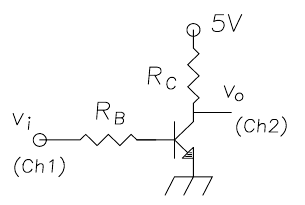
\includegraphics[width=0.5\linewidth]{image/5b}
\label{fig:5b}
\end{figure}

\begin{figure}[H]
	\centering
	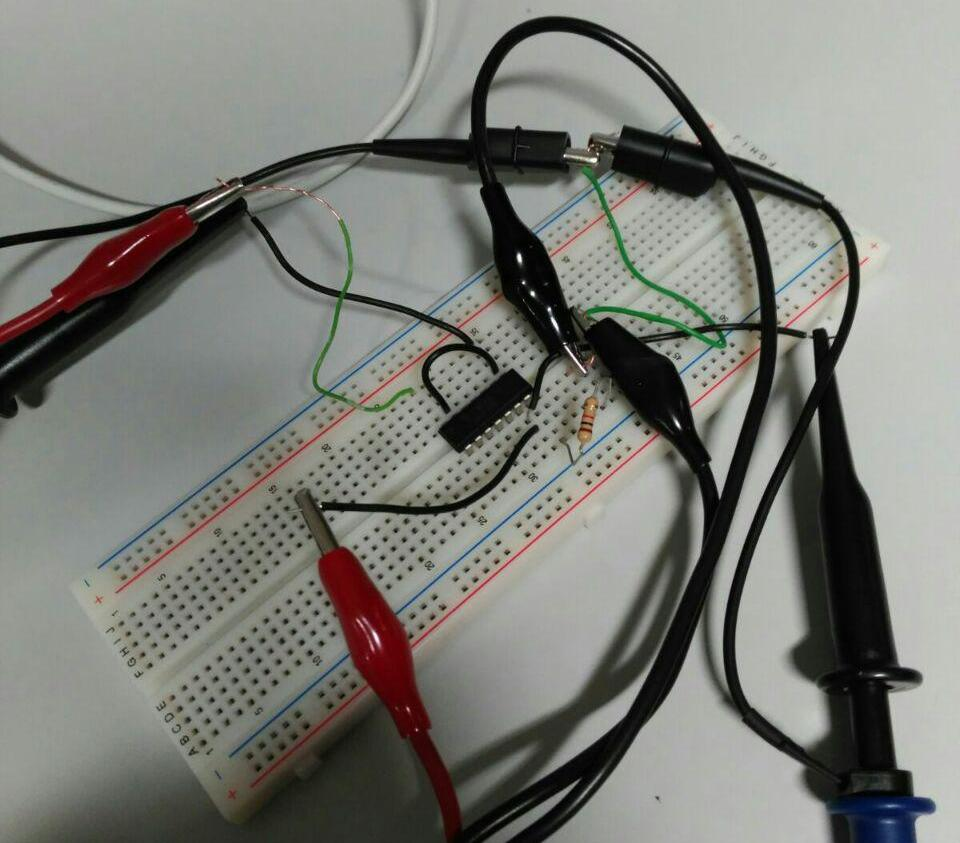
\includegraphics[scale=0.4]{image/transistorB}
	\caption{Fotografía amplificador básico}
	\label{fig:foto-transistorB}
\end{figure}

\textit{En el osciloscopio poner los dos canales en modo AC y disparar por Ch1. En [Trigger]-[Mode] poner  "Noise Reject" y "HF Reject". Es recomendable usar las medidas automáticas del osciloscopio, por eso conviene tener el disparo (trigger) bien configurado. Una vez que el montaje esté listo para medir, poner Average=4.} \newline

\textit{Deberán tomarse cuatro medidas distintas de la ganancia. La primera será con un valor $ V_{DC}=0,8V $, la última con el valor $ V_{DC} $ que haga visible en vo que el transistor entra en saturación, otra en el $ V_{DC} $ que dé la máxima ganancia, y una cuarta donde se quiera.
Deberán entregarse las imágenes (TIF) de esas cuatro medidas, y rellenar la siguiente tabla.} \newline

\begin{table}[H]
	\centering
	\begin{tabular}{|c|c|c|c|c|}
		\hline
		$ V_{DC} $ & $ V_{i}(V) $ & $ V_{0}(V) $ & $ V_{0}/V_{i} $ & Comentario \\
		\hline \hline
		0.8V & 53.5 & 198.6 & 0.2694 &  \\
		\hline
		1 V & 15.7 & 202.1 & 0.0776 &  \\
		\hline
		1.2 V & 9.8 & 199 & 0.0492 & \\
		\hline
		1.4 V & 6.7 & 97.3 & 0.6885 & Ganancia máxima \\
		\hline  
		1.8 V & - & - & - & Entra en Saturación \\
		\hline 
	\end{tabular}
	\caption{Tabla que contiene las medidas TIF}
	\label{fig:Tabla-prac-4B}
\end{table}

\newpage

\section{PRACTICA 05. Familia lógicas: CMOS}

\textit{En el circuito integrado 4007 se tienen tres mosfet de canal n y tres de canal p, por tanto se pueden construir distintas variantes de puertas CMOS. Al hacer la práctica, se debe apuntar el valor de la alimentación usada en la práctica $ (V_{CC}) $.}

\begin{figure}[H]
\centering
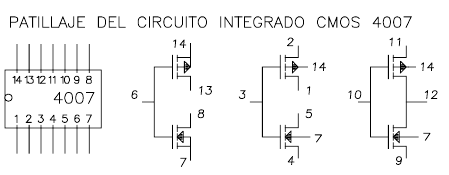
\includegraphics[width=0.7\linewidth]{image/p5a}
\end{figure}

\subsection{Puerta NOT CMOS \cite{2c}}

\begin{itemize}
	\item \textit{Construir la puerta NOT. Comprobar que los niveles de tensión de la tabla de verdad son correctos.}
	
	\begin{figure}[H]
		\centering
		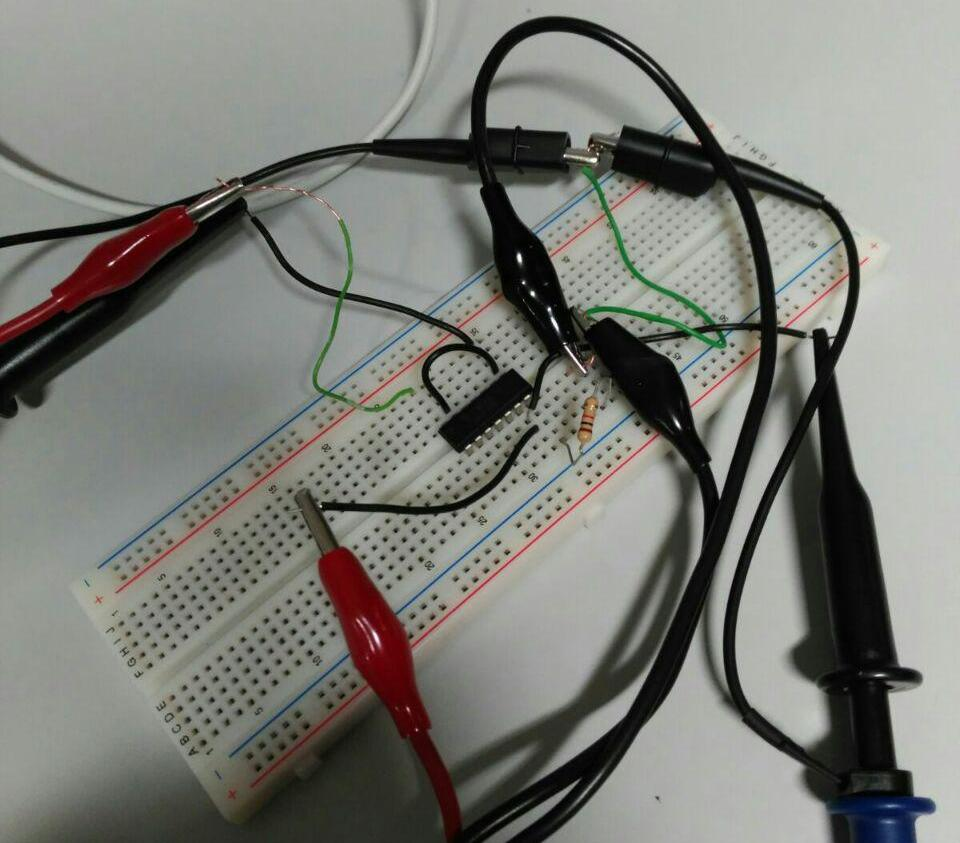
\includegraphics[scale=0.4]{image/NOT5A}
		\caption{Fotografía puerta NOT CMOS}
		\label{fig:prac-5a-notA}
	\end{figure}
	
	\item \textit{Apuntar la máxima frecuencia de trabajo admisible. Medir los retardos de bajo-alto y de alto-bajo.}
	\item \textit{Con una señal triangular (~1 kHz), medir la tensión umbral $ (V_{T}) $.}
	\item \textit{Con la anterior señal triangular, poner el modo XY del osciloscopio (Ch1 en A, Ch2 en S). Dibujar la función de transferencia. Añadir una resistencia de bajo valor $ (~100 \Omega) $ entre b y tierra. Con el osciloscopio en modo XY (Ch1 en A, Ch2 en b) dibujar la gráfica de consumo de la puerta CMOS.}
\end{itemize}

\begin{figure}[H]
	\centering
	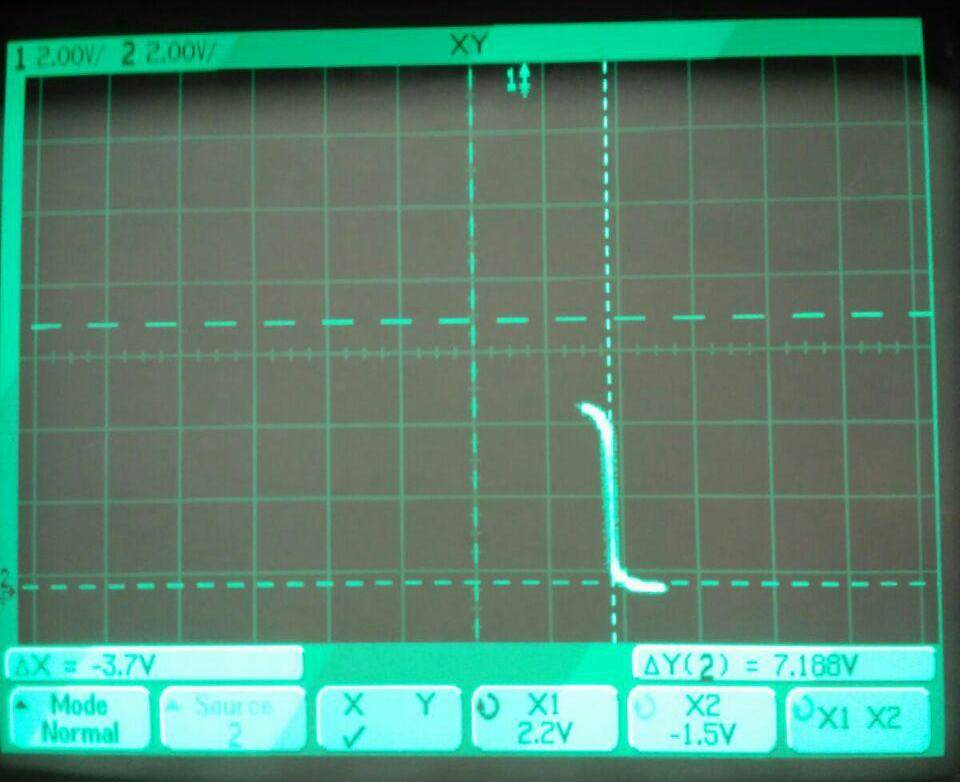
\includegraphics[scale=0.4]{image/cmos-res}
	\caption{Foto osciloscopio NOT CMOS con resistencia}
	\label{fig:prac-5a-img3a}
\end{figure}

\begin{figure}[H]
	\centering
	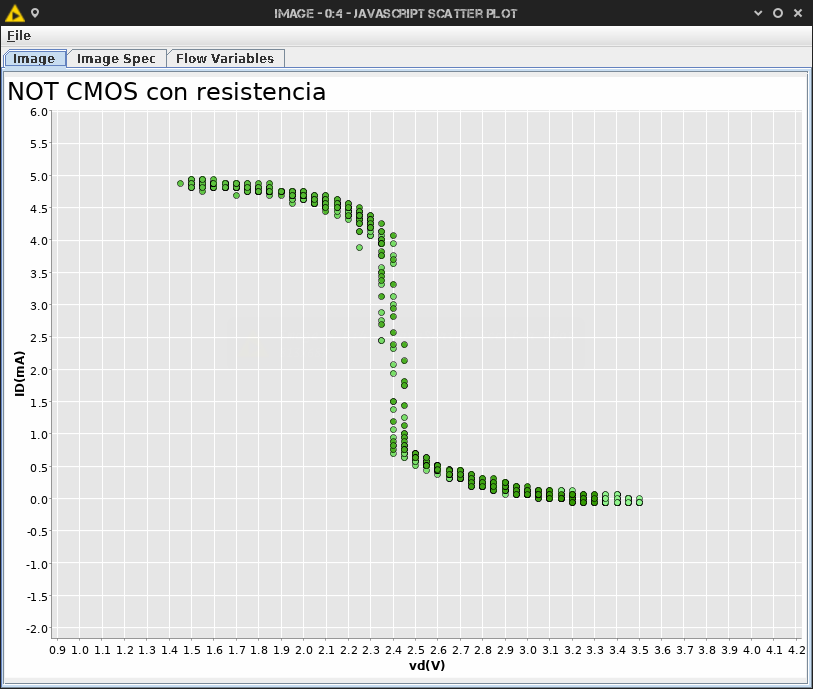
\includegraphics[scale=0.27]{image/NOTp5a}
	\caption{NOT CMOS con resistencia}
	\label{fig:prac-5a-img3}
\end{figure}

\begin{figure}[H]
	\centering
	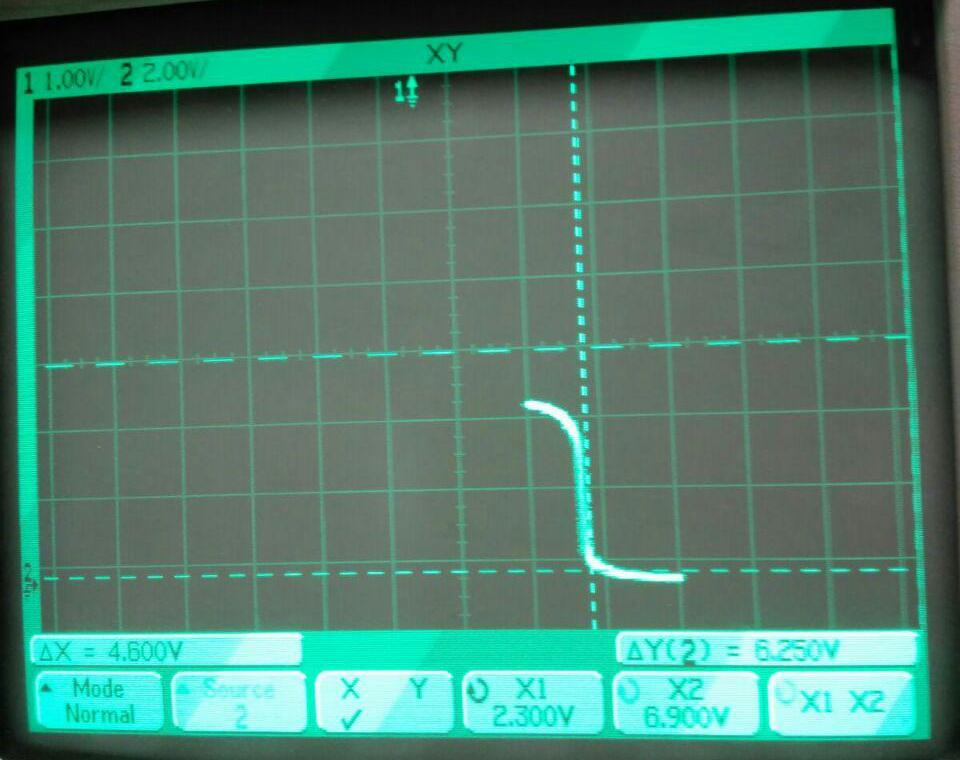
\includegraphics[scale=0.4]{image/cmos-sinres}
	\caption{Foto osciloscopio NOT CMOS sin resistencia}
	\label{fig:prac-5b-img3}
\end{figure}

\begin{figure}[H]
	\centering
	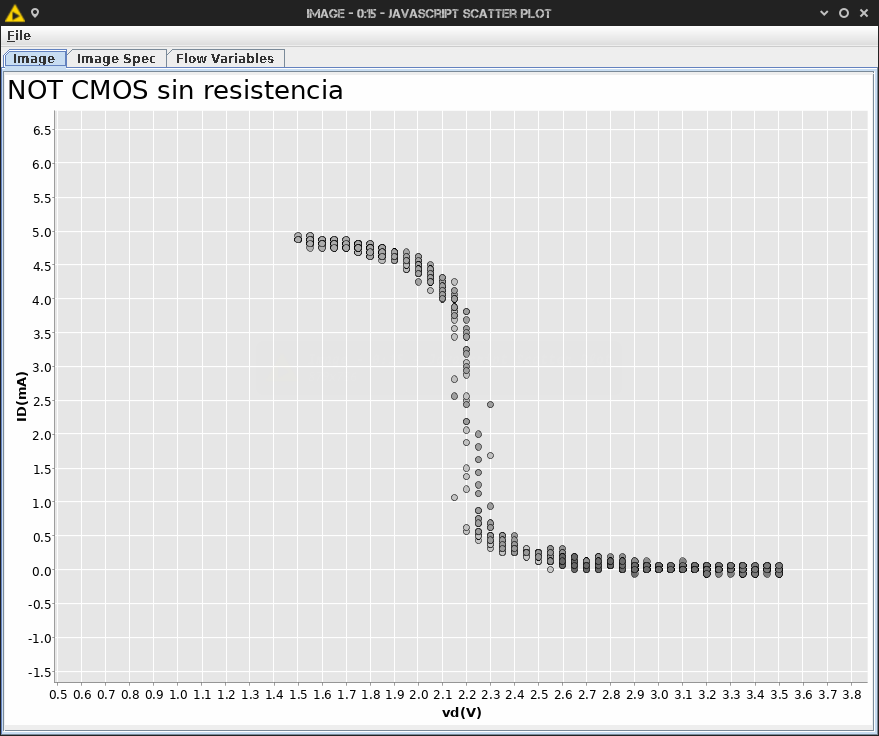
\includegraphics[scale=0.27]{image/NOTp5b}
	\caption{NOT CMOS sin resistencia}
	\label{fig:prac-5b-img3s}
\end{figure}


\subsection{Memoria CMOS \cite{RV}}

\begin{itemize}
	\item \textit{Montar la célula de memoria CMOS de la figura, con entrada A y salidas S' y S.}	
	\item \textit{Con A=0, comprobar que las salidas S' y S son correctas. Desconectar A y comprobar que S' y S se mantienen en sus valores correctos.} \newline
	
	Observamos que cuando la entrada A le entra baja (tierra) medimos el máximo voltaje del circuito como se ve en la figura 5.4.
	
	\begin{figure}[H]
		\centering
		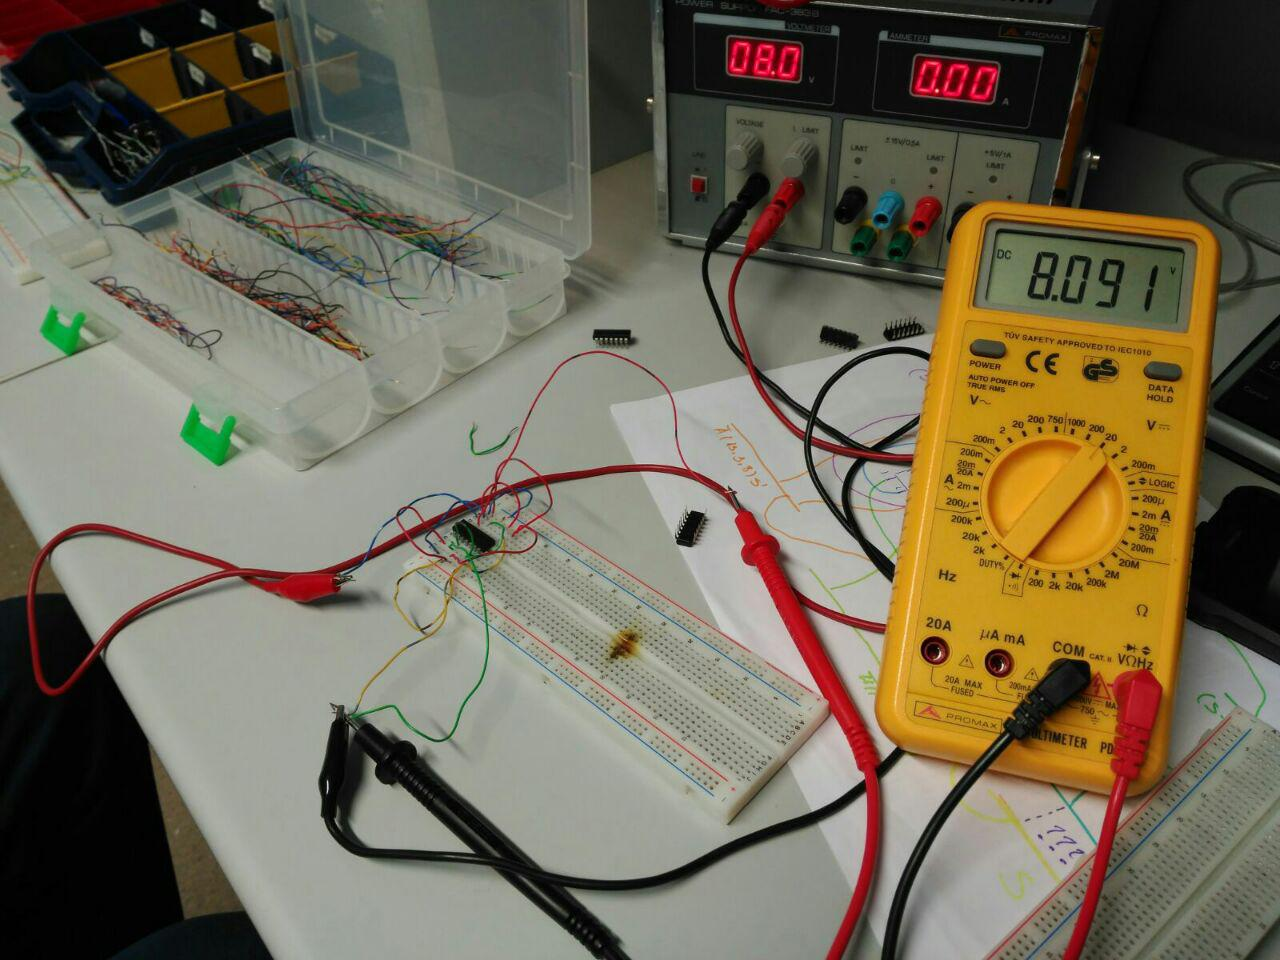
\includegraphics[scale=0.3]{image/NOT5B1}
		\caption{Foto memoria CMOS, A = 0}
		\label{fig:prac-5a-5B1}
	\end{figure}
		
	Como podemos ver el la figura 5.5 guarda el valor en memoria cuando desconectamos el tierra.
	
	\begin{figure}[H]
		\centering
		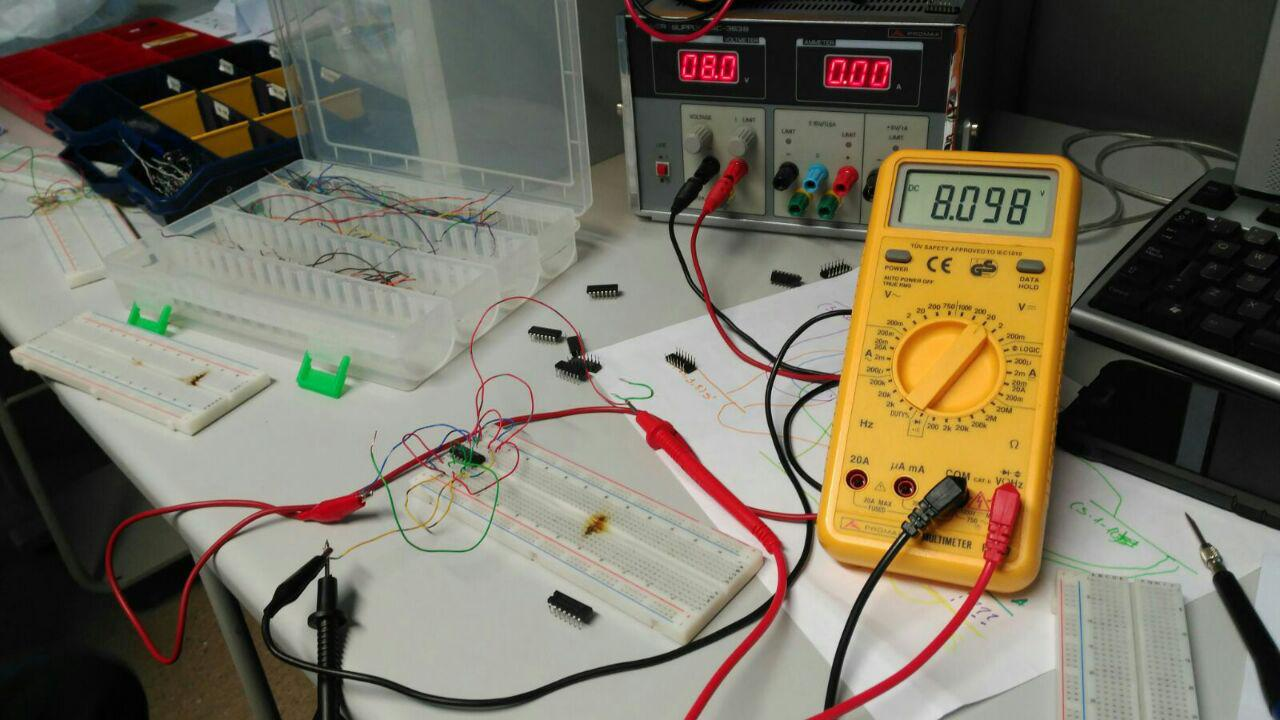
\includegraphics[scale=0.4]{image/NOT5B2}
		\caption{Foto memoria CMOS Guarda cuando A es = 0}
		\label{fig:prac-5a-5B2}
	\end{figure}
	
	\item \textit{Con A=1, comprobar que las salidas S' y S son correctas. Desconectar A y comprobar que S' y S se mantienen en sus valores correctos.} \newline
	
	Observamos que cuando la entrada A le entra alta (voltaje) medimos el mínimo voltaje del circuito como se ve en la figura 5.6.
	
	\begin{figure}[H]
		\centering
		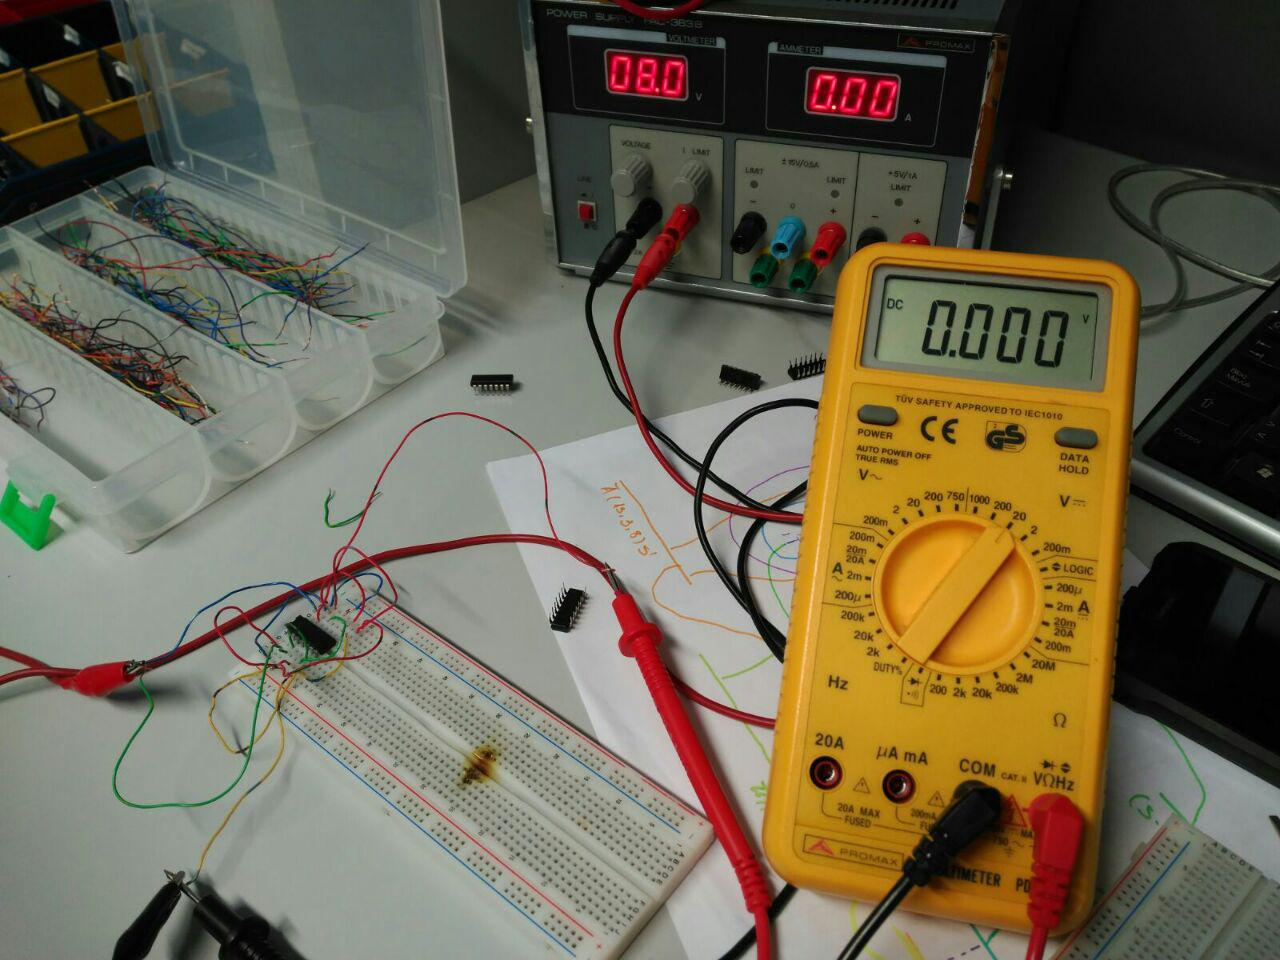
\includegraphics[scale=0.25]{image/NOT5B3}
		\caption{Foto memoria CMOS, A = 1}
		\label{fig:prac-5a-5B3}
	\end{figure}
	
	Como podemos ver el la figura 5.7 guarda el valor en memoria cuando desconectamos el voltaje.
	
	\begin{figure}[H]
		\centering
		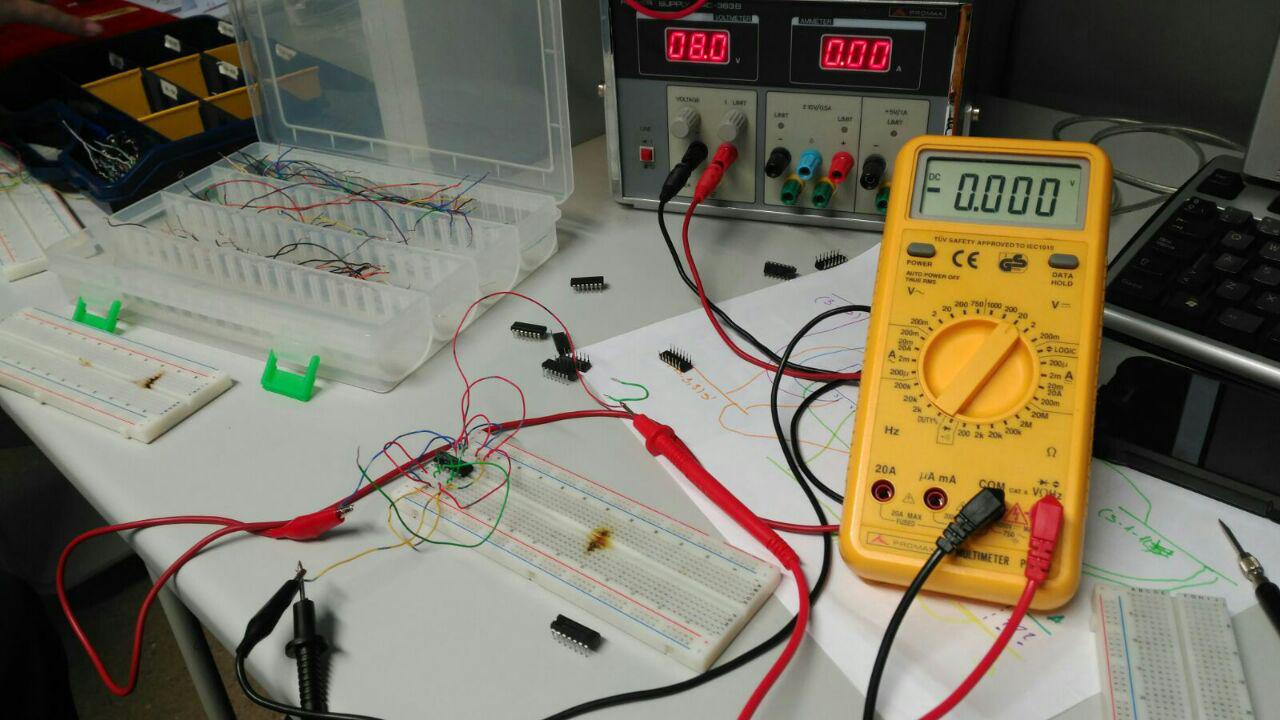
\includegraphics[scale=0.4]{image/NOT5B4}
		\caption{Foto memoria CMOS guarda cuando es A = 1}
		\label{fig:prac-5a-5B4}
	\end{figure}
\end{itemize}
 
\newpage

\section{PRACTICA 06. Conversor analógico-digital \cite{RV}}

\textit{Se va a utilizar un microcontrolador PIC12F675, que tiene un conversor analógico-digital (ADC) de 10 bits. Un microcontrolador es un ordenador contenido en un único chip, capaz de controlar totalmente tareas básicas.} \newline

\textbf{Montaje:}

\begin{itemize}
	\item \textit{La alimentación del circuito se hace poniendo $ V_{DD} $ a 5 V y $ V_{SS} $ a tierra. Entre estos dos terminales se conecta un condensador de 100 nF.}
	\item \textit{La tensión de referencia (REF) está conectada internamente a $ V_{DD} $. La tensión de referencia es la máxima tensión a digitalizar, que en este caso es la alimentación (5 V), y se debe medir con precisión.}
	\item \textit{Los 10 bits de la palabra numérica se entregan en serie (en el terminal GP0), empezando por el bit más significativo (MSB) y acabando por el menos significativo (LSB). La salida de reloj está en el terminal GP1.}
	\item \textit{La tensión analógica a digitalizar, entra en GP4, y se obtiene de la fuente de tensión variable. Si se usa el polímetro con escalas 400mV-4V, se hará con un valor por debajo de 0,4 V, y dos valores por debajo de 4 V. Si se usa el polímetro con escalas 200mV-2V, se hará con un valor por debajo de 0,2 V, y dos por debajo de 2 V.}
\end{itemize}

\begin{figure}[H]
	\centering
	\includegraphics[scale=0.45]{image/prac6A}
	\caption{Foto conversor analógico-digital}
	\label{fig:prac-5a-5B}
\end{figure}

\subsection{Actividad 1}

\textit{Medir la tensión de alimentación $ V_{DD} $ de forma muy precisa, ya que es la tensión de referencia (REF) y calcular el valor del LSB (LSB= REF / 1024).}

\subsection{Actividad 2}

Para cada tensión analógica $ (V_{a}) $:

\begin{itemize}
	\item \textit{se mide, de forma muy precisa, la tensión de entrada analógica $ V_{a} $.}
	\item \textit{se captura en un disquete la imagen (tif o bmp) del osciloscopio (datos y reloj).}
	\item \textit{se extrae de la imagen, la palabra numérica (en binario) y se convierte a decimal.}
	\item \textit{se comprueba que la palabra digital se corresponde con el valor teórico dado por la siguiente ecuación (E= función parte entera, Min= función mínimo):}
\end{itemize}

$$ Num(V_{a})=Min \; \dfrac{V_{a}+LSB/2}{LSB},1023 $$

\begin{figure}[H]
	\centering
	\includegraphics[scale=0.4]{image/prac61}
	\caption{Foto ejemplo conversor analógico-digital}
	\label{fig:prac-5a-61}
\end{figure}

\begin{table}[H]
	\centering
	\begin{tabular}{|c|c|c|c|c|c|c|c|c|}
		\hline
		\textbf{$ V_{DD} $} & \textbf{$ V_{REF} $} & \textbf{$ V $} & \textbf{$ V_{A} $ } & \textbf{LSB} &  \textbf{Binario} & \textbf{Dec} & \textbf{min\{E\{Dec\},1023\}} & Error \\
		\hline
		5 & 4.938 & 1.6 & 1.63 & 0.00482226 & 0101010011 & 339 & 338 & 1 \\
		\hline
		5 & 4.938 & 0.7 & 0.775 & 0.00482226 & 0010100010 & 162 & 161 & 1 \\
		\hline
		5 & 4.938 & 0.2 & 0.238 & 0.00482226 & 0000110011 & 51 & 49 & 2 \\
		\hline
	\end{tabular}
	\caption{Valores tomados en clase.} \label{medidas}
\end{table}

En el ultimo caso debido a un aumento de ruido obtuvimos un bit mas de error ademas del bit que siempre obtenemos por el fabricante.

\newpage

\section{PRACTICA 07. Conservor analógico-digital - SUBIR NOTA \cite{RV}}


\textbf{Montaje:}

\begin{itemize}
	\item \textit{Sin conectar el USB al ordenador, sin establecer conexión con el teléfono, montar el circuito, pero inicialmente conectar GP3 a 5 V, ya que en esa posición el 10F222 emitirá la cadena de caracteres "0123456789ABCDEF" que servirá para probar si la transmisión hacia el ordenador está libre de problemas. El cable amarillo de (TXD/TX>) no debe dejarse suelto, pues un movimiento puede provocar un cortocircuito; conectarlo a un agujero sin uso de la placa de conexiones. Revisar el circuito meticulosamente.}
	\item \textit{[USB] Conectar el circuito USB al ordenador. Para recibir las palabras digitales, los valores numéricos de la tensión analógica, usaremos el comando xxd. Con el comando xxd </dev/ttyUSB0, los valores numéricos recibidos en el puerto USB, se transforman en tabla de valores hexadecimales legibles en la pantalla del ordenador.}
	\item \textit{[BT] Establecer conexión entre el programa terminal BT en Android, con el módulo BT del montaje.
		En el terminal se verán los valores numéricos recibidos en hexadecimal.}
	\item \textit{Para ver la transmisión de los datos en TTL-232, conectar el canal-1 del osciloscopio en GP1. Pulsar [Edge] y poner en flanco descendente para detectar el bit de "Start" en el canal-1. Es necesario utilizar el modo normal de disparo [Mode-Coupling]-[Normal], no el automático.}
\end{itemize}

\begin{figure}[H]
\centering
\includegraphics[width=1\linewidth]{image/p7}
\label{fig:p7}
\end{figure}

\subsection{Atividad 1}

\textit{Medir la tensión de alimentación en el potenciómetro (VREF) de forma precisa, y calcular el valor del LSB (LSB= VREF / 256). Poner GP3 a 0 V.}

\subsection{Atividad 2}

\textit{Si se usa el polímetro con escalas 400mV-4V, se digitalizará un valor por debajo de 0,4 V, y dos valores por debajo de 4 V. Si se usa el polímetro con escalas 200mV-2V, se hará con un valor por debajo de 0,2 V, y dos por debajo de 2 V. Para estos tres valores de $ V_{a} $:}

\begin{itemize}
	\item \textit{Se mide, de forma precisa, la tensión de entrada Va. Se calcula el valor decimal $ Num(V_{a}) $ con la siguiente ecuación (E= función parte entera, Min= función mínimo):}
	\item \textit{Se captura en un disquete la imagen (tif o bmp) del osciloscopio. Se extrae de la imagen la palabra numérica en binario, y se pasa a decimal.}
	\item \textit{Se apunta la palabra en hexadecimal recibida en el ordenador, y se pasa a decimal.}
\end{itemize}

\textit{Finalmente se comprueba que los valores decimales de la fórmula teórica, de la imagen del osciloscopio, y del valor hexadecimal recibido en el ordenador coinciden.}

\begin{figure}[H]
	\centering
	\includegraphics[scale=0.4]{image/prac7A}
	\caption{Foto memoria CMOS}
	\label{fig:prac-5a-7B}
\end{figure}

Montamos el circuito tal y como se muestra en la figura. Conectamos el terminal del bluetooth. Intentamos conectarlo al ordenador pero en linux nos producía errores de permisos, por lo tanto usamos un móvil con android y la aplicación bluetooth terminal. \newline

\begin{figure}[H]
	\centering
	\includegraphics[scale=0.6]{image/prac71}
	\caption{Foto conversor analógico-digital}
	\label{fig:prac-5a-71}
\end{figure}

Sincronizamos el móvil con el dispositivo bluetool del circuito y como vemos en la figura 7.2 comenzamos a recibir datos en hexadecimal y ademas recibimos una señal que nos proporciona una palabra en binario que coincidía con la recibida en hexadecimal en el móvil. \newline

En la practica procedemos a leer el numero en binario del osciloscopio, pasarlo a decimal y con la formula que nos proporciona la práctica obtenemos los siguientes resultados: \newline

\begin{table}[H]
	\centering
	\begin{tabular}{|c|c|c|c|c|c|c|c|c|c|}
		\hline
		\textbf{$ V_{DD} $} & \textbf{$ V_{REF} $} & \textbf{$ V $} & \textbf{$ V_{A} $ } & \textbf{LSB} &  \textbf{Binario} & \textbf{Dec} & \textbf{Hex} & \textbf{min\{E\{Dec\},255\}} & Error \\
		\hline
		5 & 8.106 & 1.8 & 1.833 & 0.020023529 & 1011010 & 90 & 5A & 89 & 1 \\
		\hline
	\end{tabular}
	\caption{Valores tomados en clase.} \label{medidas}
\end{table}

\newpage

\section{Tiristores. EXTRA}

Como podemos ver en las imágenes al apagar el tiristor obtenemos mayor luminosidad. \newline


\begin{figure}[H]
	\centering
	\includegraphics[scale=0.7]{image/practica1-bombillaA}
	\caption{Fotografía con tiristor encendido.} \label{Color-resistencia}
\end{figure}

\begin{figure}[H]
	\centering
	\includegraphics[scale=0.7]{image/practica1-bombillaB}
	\caption{Fotografía fotografia con tiristor apagado.} \label{Color-resistencia}
\end{figure}

%----------------------------------------------------------------------------------------
%	Bibliografía y citas
%----------------------------------------------------------------------------------------

\vspace*{13cm}

\bibliography{citas} %archivo citas.bib que contiene las entradas 
\bibliographystyle{plain} % hay varias formas de citar

\end{document}
